% species names
\newcommand{\dicty}{\emph{D.~discoideum}}

% gene names
\newcommand{\nlp}{\gene{nlp-31}}
\newcommand{\ftna}{\gene{ftn-1}}
\newcommand{\ftnb}{\gene{ftn-2}}
\newcommand{\cysl}{\gene{cysl-1}}
\newcommand{\nog}{\gene{nog-1}}
\newcommand{\nhr}{\gene{nhr-57}}
\newcommand{\lam}{\gene{lam-3}}
\newcommand{\fog}{\gene{fog-2(lf)}}
\newcommand{\egl}{\gene{egl-9(lf)}}
\newcommand{\rhy}{\gene{rhy-1(lf)}}
\newcommand{\vhl}{\gene{vhl-1(lf)}}
\newcommand{\eglvhl}{\gene{egl-9(lf); vhl-1(lf)}}
\newcommand{\eglhif}{\gene{egl-9(lf) hif-1(lf)}}
\newcommand{\hif}{\gene{hif-1(lf)}}

% protein names
\newcommand{\eglp}{EGL-9}
\newcommand{\rhyp}{RHY-1}
\newcommand{\nogp}{NOG-1}
\newcommand{\vhlp}{VHL-1}
\newcommand{\hifp}{HIF-1}
\newcommand{\fogp}{FOG-2}
\newcommand{\nhrp}{NHR-57}
\newcommand{\lamp}{LAM-3}
\newcommand{\cyslp}{CYSL-1}

% DE genes numbers:
\newcommand{\egln}{2,549}
\newcommand{\rhyn}{3,005}
\newcommand{\vhln}{1,275}
\newcommand{\eglvhln}{3,654}
\newcommand{\hifn}{1,075}
\newcommand{\eglhifn}{744}
\newcommand{\fogn}{2,840}
\newcommand{\total}{7,609}

% downstream targets
\newcommand{\egltargets}{4}
\newcommand{\rhytargets}{0}
\newcommand{\vhltargets}{71} % 72 minus vhl-1 (IDed due to deletion)
\newcommand{\hiftargets}{264}
\newcommand{\hifohtargets}{56}

% website commands
\newcommand{\website}{
            \url{https://wormlabcaltech.github.io/mprsq/}
            }
\newcommand{\webref}{
\href{https://wormlabcaltech.github.io/mprsq/}{website}}

% more space between rows
\newcommand{\ra}[1]{\renewcommand{\arraystretch}{#1}}

% \title{Reconstructing a metazoan genetic pathway with transcriptome-wide epistasis
%        measurements}
% \author[a, b, 1]{David Angeles-Albores}
% \author[a, b, c, 1]{Carmie Puckett Robinson}
% \author[a]{Brian A. Williams}
% \author[a]{Barbara J. Wold}
% \author[a, b]{Paul W. Sternberg}
%
% \affil[a]{Division of Biology and Biological Engineering, Caltech, Pasadena, CA,
%          91125, USA}
% \affil[b]{Howard Hughes Medical Institute, Caltech, Pasadena, CA, 91125, USA}
% \affil[c]{Department of Neurology, Keck School of Medicine, University of
%          Southern California, Los Angeles, California, 90033, USA}



\section*{Abstract}
\textbf{
RNA-seq is commonly used to identify genetic modules that respond to
perturbations. In single cells, transcriptomes have been used as phenotypes,
but this concept has not been applied to whole-organism RNA-seq. Also,
quantifying and interpreting epistatic effects using expression profiles
remains a challenge. We developed a single coefficient to quantify
transcriptome-wide epistasis that reflects the underlying interactions and
which can be interpreted intuitively. To demonstrate our approach, we
sequenced four single and two double mutants of \emph{Caenorhabditis~elegans}.
From these mutants, we reconstructed the known hypoxia pathway. In addition,
we uncovered a class of \hifohtargets{} genes with \gene{hif-1}-dependent
expression that have opposite changes in expression in mutants of two genes
which cooperate to negatively regulate \hifp{} abundance; however, the double
mutant of these genes exhibits suppression epistasis. This class violates the
classical model of HIF-1 regulation, but can be explained by postulating a
role of hydroxylated HIF-1 in transcriptional control.
}
\vspace{10mm}


\section*{Introduction}
\label{sec:introduction}
Genetic analysis of molecular pathways has traditionally been performed through
epistatic analysis. If the mutants of two distinct genes have a quantifiable
phenotype, and the double mutant has a phenotype that is not the sum of the
phenotypes of the single mutants, this non-additivity is referred to as
generalized epistasis, and indicates that these genes interact functionally.
Such interactions can occur at the biochemical  level between their products or
as a consequence of their functions~\citep{Huang2006}. Epistasis analysis remains
a cornerstone of genetics today~\citep{Phillips2008}.

Recently, biological studies have shifted in focus from studying single genes to
studying all genes in parallel. In particular, RNA-seq~\citep{Mortazavi2008}
enables biologists to identify genes that change expression in response to a
perturbation. RNA-seq has been used to identify genetic modules involved in a
variety of processes, such as in the \emph{Caenorhabditis~elegans} linker cell
migration~\citep{Schwarz2012}, planarian stem cell
maintenance~\citep{VanWolfswinkel2014,Scimone2014}. The role of transcriptional
profiling has been restricted to target gene identification, and so far there
are only a few examples where transcriptomes have been used to generate
quantitative genetic models of any kind. In quantitative genetics, eQTL studies
have established the power of transcriptomes for genetic
mapping~\citep{Brem2002,Schadt2003,Li2006,King2014}. Genetic pathway analysis via
epistasis has been performed in
\emph{Saccharomyces~cerevisiae}~\citep{Hughes2000,Capaldi2008} and in
\emph{Dictyostelium~discoideum}~\citep{VanDriessche2005}. Recently, Dixit
\emph{et al} described a protocol for epistasis analysis in dendritic and K562
cells using single-cell RNA-seq~\citep{Dixit2016}. Epistasis analysis of single
cells or single-celled organisms is popular because of the concern that
whole-organism sequencing will mix information from multiple cell types,
preventing the accurate reconstruction of genetic interactions. Using
whole-organism transcriptome profiling, we have recently identified a new
developmental state of \cel{} caused by loss of a single cell type (sperm
cells)~\citep{Angeles-Albores2017}, which suggests that whole-organism
transcriptome profiling contains sufficient information for epistatic analysis.
To investigate the ability of whole-organism transcriptomes to serve as
quantitative phenotypes for epistatic analysis in metazoans, we sequenced the
transcriptomes of four well-characterized loss-of-function mutants in the \cel{}
hypoxia pathway~\citep{Epstein2001,Shen2006,Shao2009,Jiang2001}.

% carmie:
Metazoans depend on the presence of oxygen in sufficient concentrations to
support aerobic metabolism. Hypoxia inducible factors (HIFs) are an important
group of oxygen-responsive genes that are highly conserved in
metazoans~\citep{Loenarz2011}. A common mechanism for hypoxia-response induction
is heterodimerization between a HIF$\alpha$ and a HIF$\beta$ subunit; the
heterodimer then initiates transcription of target genes~\citep{Jiang1996}. The
number and complexity of HIFs varies throughout metazoans. In the roundworm
\cel{} there is a single HIF$\alpha$ gene, \gene{hif-1}~\citep{Jiang2001}, and a
single HIF$\beta$ gene, \gene{ahr-1}~\citep{Powell-Coffman1998}.

Levels of HIF$\alpha$ proteins are tightly regulated. Under conditions of
normoxia, \hifp{}$\alpha$ exists in the cytoplasm and partakes in a futile cycle
of protein production and rapid degradation~\citep{Huang1996}. In \cel{},
\hifp{}$\alpha$ is hydroxylated by a proline hydroxylase
(\eglp{})~\citep{Kaelin2008}. \hifp{} hydroxylation increases its binding
affinity to Von Hippel-Lindau tumor suppressor 1 (\vhlp{}), which in turn allows
ubiquitination of \hifp{} leading to its degradation. In \cel{}, \eglp{}
activity is inhibited by binding of \cyslp{}, a homolog of
sulfhydrylases/cysteine synthases; and \cyslp{} activity is in turn inhibited by
the putative transmembrane O-acyltransferase \rhyp{}, possibly by
post-translational modifications to \cyslp{}~\citep{Ma2012} (see
Fig.~\ref{fig:pathway}).

\begin{figure}[tbhp]
  \centering
  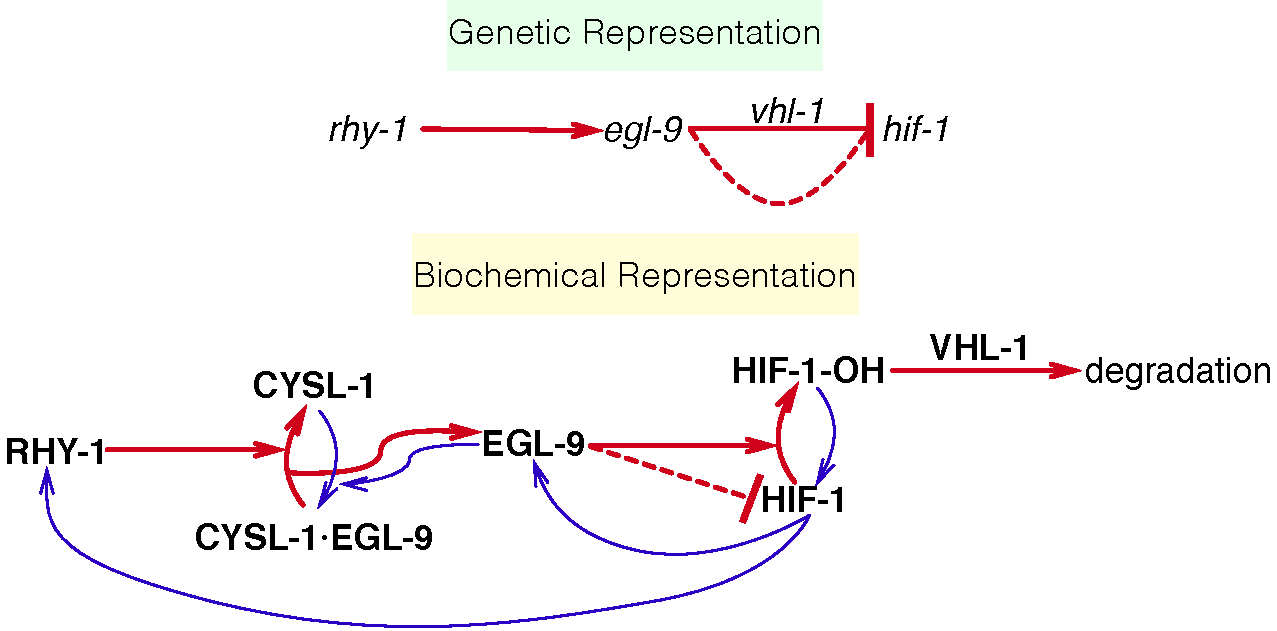
\includegraphics[width=\textwidth]{hypims/HIF1pathway.pdf}
  \caption{
    Genetic and biochemical representation of the hypoxia pathway in \cel{}. Red
    arrows are arrows that lead to inhibition of \hifp{}, and blue arrows are
    arrows that increase \hifp{} activity or are the result of \hifp{} activity.
    \eglp{} is known to exert \vhlp{}-dependent and independent repression
    on \hifp{} as shown in the genetic diagram. The \vhlp{}-independent
    repression of \hifp{} by \eglp{} is denoted by a dashed line and is not
    dependent on the hydroxylating activity of \eglp{}. RHY-1
    inhibits CYSL-1, which in turn inhibits EGL-9, but this interaction was
    abbreviated in the genetic diagram for clarity.
  }
\label{fig:pathway}
\end{figure}

Our reconstruction of the hypoxia pathway in \cel{} shows that whole-animal
transcriptome profiles can be used as phenotypes for genetic analysis and that
epistasis, a hallmark of genetic interaction observed in double mutants, holds
at the molecular systems level. We demonstrate that transcriptomes can aid in
ordering genes in a pathway using only single mutants. We were able to identify
genes that appear to be downstream of \gene{vhl-1}, but not downstream of
\gene{hif-1}. Using a single set of transcriptome-wide measurements, we observed
most of the known transcriptional effects of \gene{hif-1} as well as novel
effects not described before in \cel{}. Taken together, this analysis
demonstrates that whole-animal RNA-seq is a fast and powerful method for genetic
analyses in an area where phenotypic measurements are now the rate-limiting
step.

\section*{Results}
\subsection*{The hypoxia pathway controls thousands of genes in \cel{}}
\label{sub:summary}

We selected four null single mutants within the hypoxia pathway for expression
profiling: \gene{egl-9(sa307)}, \gene{rhy-1(ok1402)}, \gene{vhl-1(ok161)},
\gene{hif-1(ia4)}. We also sequenced the transcriptomes of two double mutants,
\gene{egl-9; vhl-1} and \gene{egl-9 hif-1} as well as wild type (N2).
Each genotype was sequenced in triplicate using mRNA extracted from 30 worms at
a depth of 15~million reads per sample. Of these 15~million reads, 50\% of the
reads mapped to the \cel{} genome on average. All samples were analyzed under
normoxic conditions.
We measured differential expression of 19,676 isoforms across all replicates and
genotypes ($\sim$70\% of the protein coding isoforms in \cel{}; see
\href{https://wormlabcaltech.github.io/mprsq/analysis_notebooks/1_basic_stats.html}
{Basic Statistics Notebook}). We included in our analysis a \gene{fog-2(q71)}
mutant we have previously studied~\citep{Angeles-Albores2017}, because
\gene{fog-2} is not reported to interact with the hypoxia pathway. We analyzed
our data using a general linear model on logarithm-transformed counts. Changes
in gene expression are reflected in the regression coefficient $\beta$, which is
specific to each isoform within a genotype (excluding wild type, which is used
as baseline). Statistical significance is achieved when the q-value of a $\beta$
coefficient ($p$-values adjusted for multiple testing) are less than 0.1.
Transcripts that are differentially expressed between the wild type and a given
mutant have $\beta$ values that are statistically significantly different from 0
(i.e.\ greater than 0 or less than 0). $\beta$ coefficients are analogous to the
logarithm of the fold-change between the mutant and the wild type. Larger
magnitudes of $\beta$ correspond to larger perturbations (see
Fig.~\ref{fig:explain}). When we refer to $\beta$ coefficients and $q$-values,
it will always be in reference to isoforms. However, we report the sizes of each
gene set by the number of differentially expressed genes (DEGs), not isoforms,
they contain. For the case of \cel{}, this difference is negligible since the
great majority of protein-coding genes have a single isoform. We have opted for
this method of referring to gene sets because it simplifies the language
considerably. A complete version of the code used for this analysis with ample
documentation, is available at \url{https://wormlabcaltech.github.io/mprsq}.


\begin{figure}[tbhp]
  \centering
  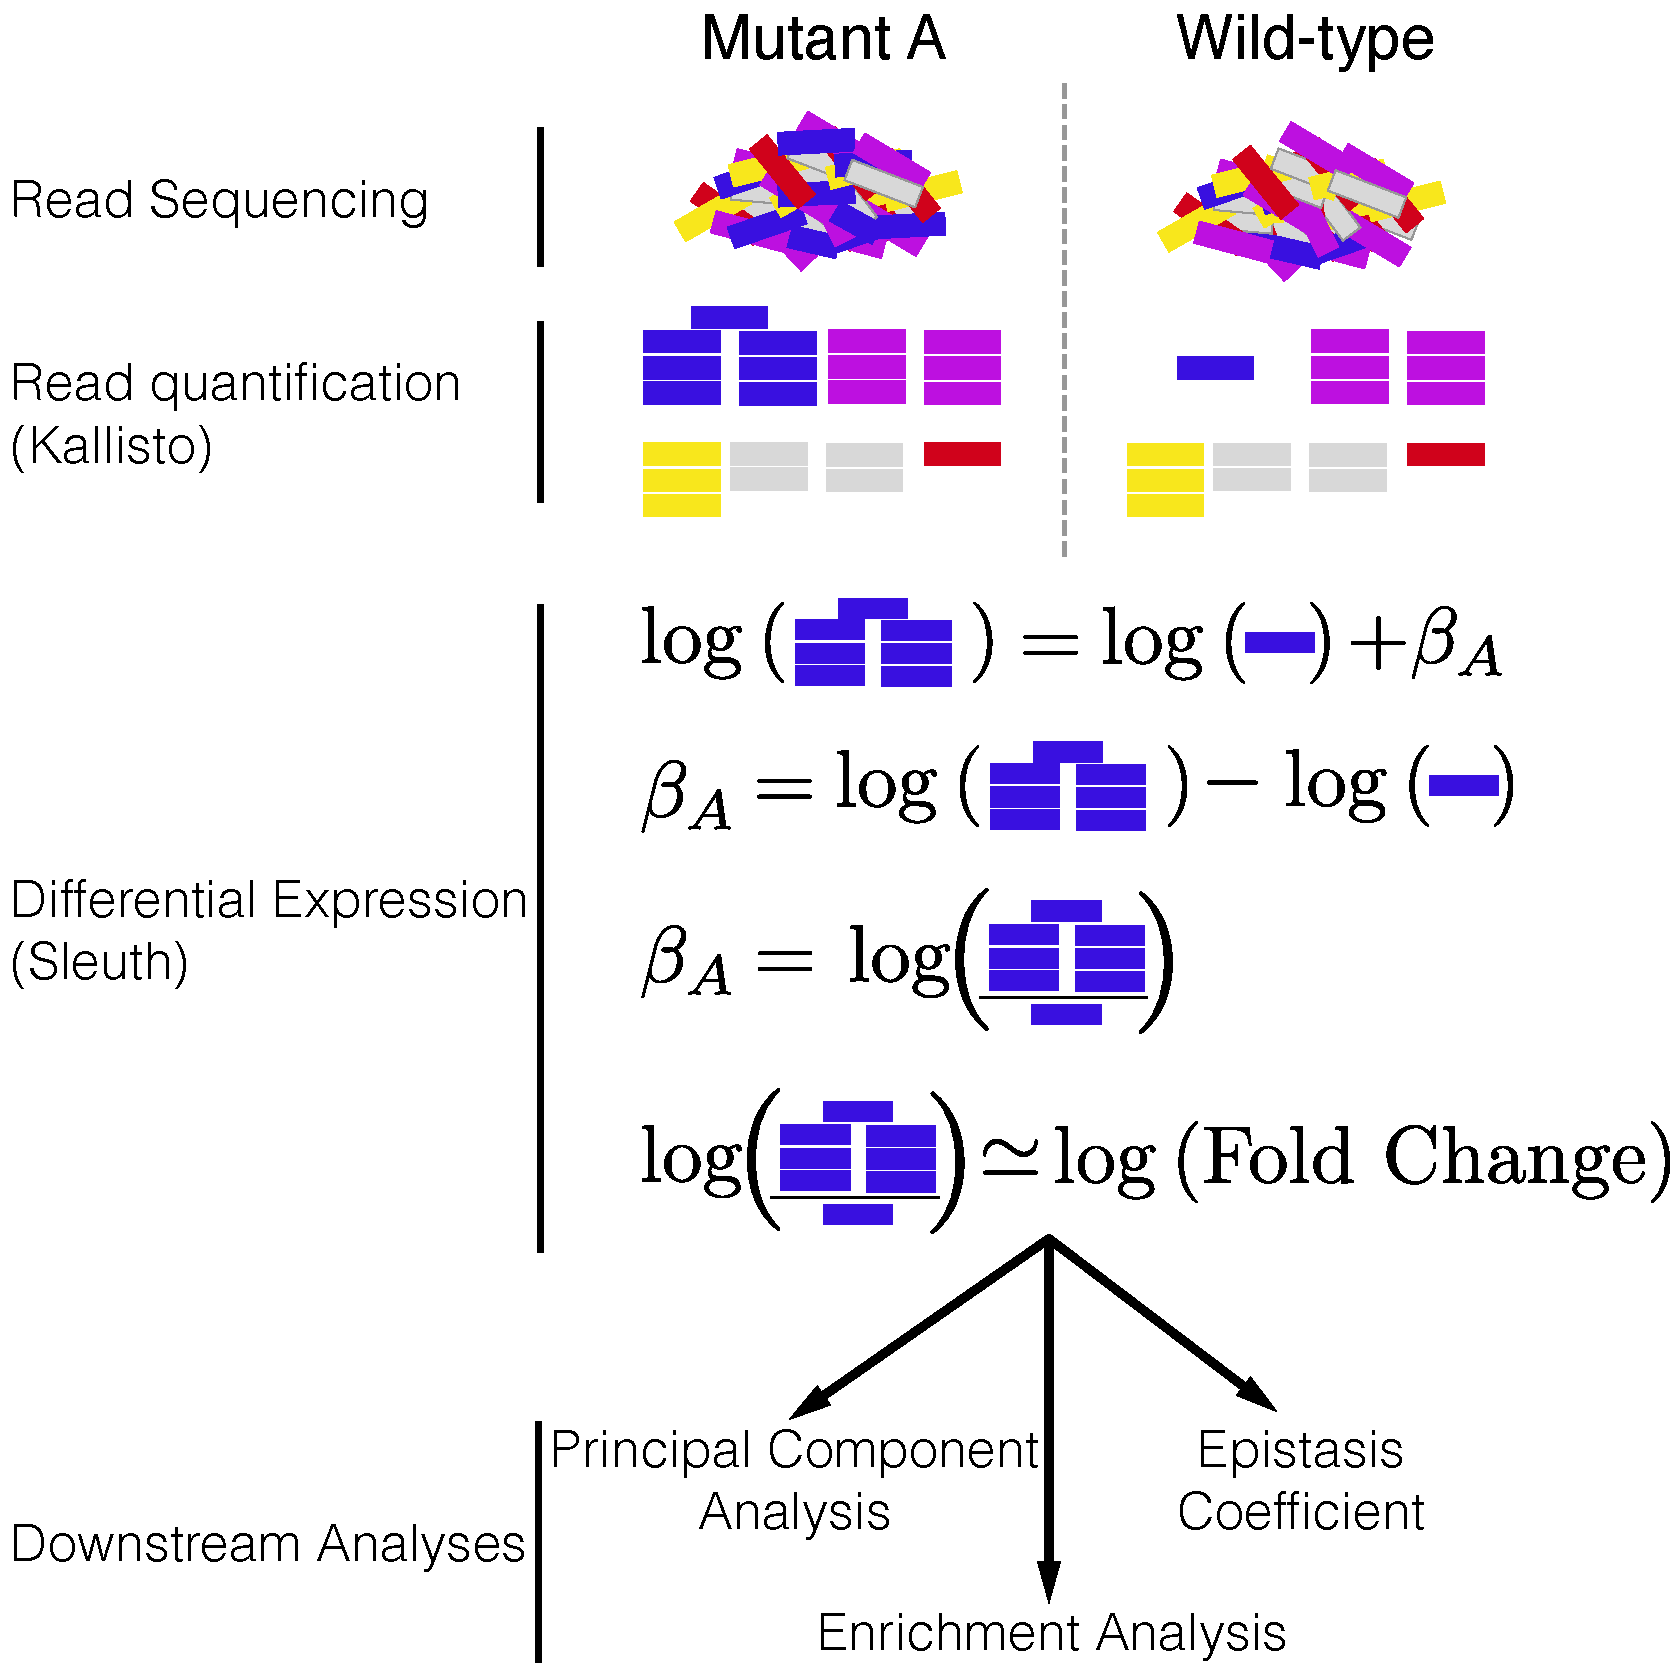
\includegraphics[width=\textwidth]{hypims/meaningofbeta.pdf}
  \caption{
    Analysis workflow. After sequencing, reads are quantified using Kallisto.
    Bars show estimated counts for each isoform. Differential expression is
    calculated using Sleuth, which outputs one $\beta$ coefficient per isoform
    per genotype. $\beta$ coefficients are analogous to the natural logarithm of
    the fold-change relative to a wild type control. Downstream analyses are
    performed with $\beta$ coefficients that are statistically significantly
    different from 0. $q$-values less than 0.1 are considered statistically
    different from 0.
  }
\label{fig:explain}
\end{figure}

Transcriptome profiling of the hypoxia pathway revealed that this pathway
controls thousands of genes in \cel{} (see Table~\ref{tab:genes}, see
SI File 1 for a complete list of differentially expressed genes).
The \egl{}
transcriptome showed differential expression of \egln{} genes. \rhyn{} genes
were differentially expressed in \rhy{} mutants. The \vhl{} transcriptome showed
considerably fewer DEGs (\vhln{}), possibly because \gene{vhl-1} is a weaker
inhibitor of \gene{hif-1} than \gene{egl-9}~\citep{Shao2009}. The \egl{};\vhl{}
double mutant transcriptome showed \eglvhln{} DEGs. The \hif{} mutant showed a
transcriptomic phenotype involving \hifn{} genes. The \eglhif{} double mutant
showed a similar number of genes with altered expression (\eglhifn{} genes).
We do not think that this transcriptional response is the due to transiently
induced hypoxia during harvesting. If the wild type strain had become hypoxic,
then the \hif{} genotype should show significantly lower levels of
\gene{nhr-57}, a marker that increases during hypoxia. We do not observe altered
levels of \gene{nhr-57} when comparing the wild type and \hif{} mutant, nor
between the wild type and \eglhif{} double mutant. Finally, the \egl{}, \vhl{},
\rhy{} and \eglvhl{} mutants did show altered \gene{nhr-57} transcript levels
(see
\href{https://wormlabcaltech.github.io/mprsq/analysis_notebooks/5_quality_check.html}{
Quality Control Notebook}, SI Figure 1). Of the differentially expressed genes
in \hif{} mutants, 161/\hifn{} were also differentially expressed in \eglhif{}
mutants, which suggests these transcripts are \gene{hif-1}-dependent under
normoxia. For the remaining genes, we cannot rule out cumulative effects from
loss of \gene{hif-1}, strain-specific eQTLs present in the strain background or
that loss of \gene{egl-9} suppresses the mutant phenotype. We designed our
experiments to probe the constitutive hypoxia response, and not the effects of
\gene{hif-1} under normoxia, which we did not foresee. As a result, we have
limited resolving power to explain the transcriptome of \hif{} mutants.

\begin{table}[tbhp]
  \centering
  \begin{tabular}{lr}
    \toprule{}
    Genotype & Differentially Expressed Genes\\
    \midrule{}\egl{} & \egln{}\\
    \rhy{} & \rhyn{}\\
    \vhl{} & \vhln{}\\
    \hif{} & \hifn{}\\
    \eglvhl{} & \eglvhln{}\\
    \eglhif{} & \eglhifn{}\\
    \fog{} & \fogn{}\\
    \bottomrule{}
  \end{tabular}
  \caption{Number of differentially expressed genes in each mutant strain with
  respect to the wild type (N2).}
\label{tab:genes}
\end{table}

\subsection*{Principal Component Analysis visualizes epistatic relationships
             between genotypes}
\label{sub:Clustering}

Principal component analysis (PCA) is used to identify relationships between
high-dimensional data points~\citep{Yeung2001}. We used PCA
examine whether each genotype clustered in a biologically relevant manner. PCA
identifies the vector that explains most of the variation in the data; this
is called the first principal component. PCA can identify the first
$n$ components that explain more than 95\% of the data variance.
Clustering in these $n$ dimensions can indicate biological
relationships, although interpreting principal components can be
difficult.
% After applying PCA, we expected \hif{} to cluster near \eglhif{}, because
% \hif{} exhibits no phenotypic defects under normoxic conditions, in contrast to
% \egl{}, which exhibits an egg-laying (Egl) phenotype in the same environment.
% In \eglhif{} mutants the Egl phenotype of \egl{} mutants is suppressed and instead
% the grossly wild-type phenotype of \hif{} is observed. On the other hand, we
% expected \egl{}, \rhy{}, \vhl{} and \eglvhl{} to form a separate cluster since
% each of these genotypes is Egl and has a constitutive hypoxic response. Finally,
% we included as a negative control a \fog{} mutant we have analyzed
% previously~\citep{Angeles-Albores2016a}. This data was obtained at a different
% time from the other genotypes, so we included a batch-normalization term in our
% equations to account for this. Since \gene{fog-2} has not been described
% to interact with the hypoxia pathway, we expected that it should appear far away
% from either cluster.
In our analysis, the first principal component discriminated mutants
that have constitutive high levels of \hifp{} from mutants that have no \hifp{},
whereas the second component was able to discriminate between mutants within the
hypoxia pathway and outside the hypoxia pathway (see Fig.~\ref{fig:pca};
\gene{fog-2} is not reported to act in the hypoxia pathway and acts as a
negative control; see
\href{https://wormlabcaltech.github.io/mprsq/analysis_notebooks/2_predict_interactions.html}
{Genetic Interactions Notebook}).
% Therefore, expression profiling measures enough signal to
% cluster genes in a meaningful manner in complex metazoans.

\begin{figure}[tbhp]
  \centering
  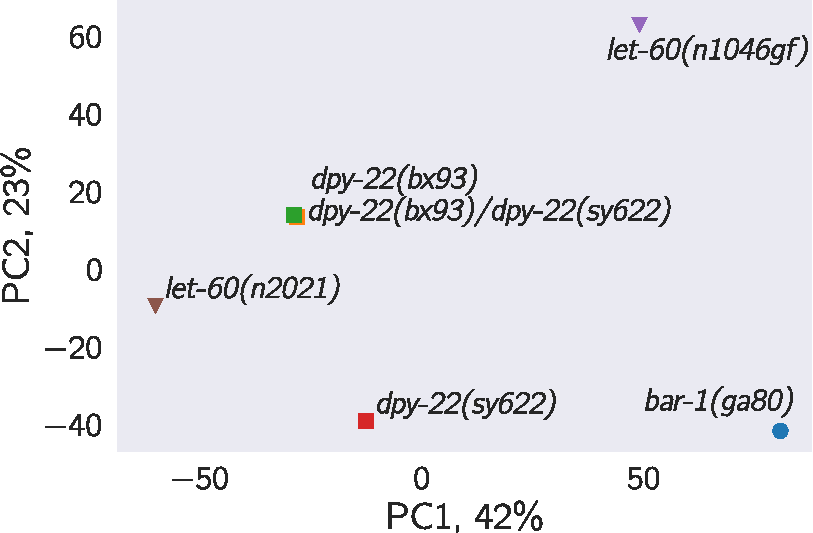
\includegraphics[width=\textwidth]{hypims/pca.pdf}
  \caption{
    Principal component analysis of various \cel{} mutants. Genotypes that have
    an constitutive hypoxia response (i.e. \egl{}) cluster far from genotypes
    that do not have a hypoxic response (i.e. \hif{}) along the first principal
    component. The second principal component separates genotypes that do not
    participate hypoxic response pathway.
  }
\label{fig:pca}
\end{figure}

\subsection*{Reconstruction of the hypoxia pathway from first genetic principles}
\label{sec:reconstruct}
To reconstruct a genetic pathway, we must assess whether two genes act on
the same phenotype. If they do not act on the same phenotype (two mutations do
not cause the same genes to become differentially expressed relative to
wild type), these mutants are independent. Otherwise, we must measure whether
these genes act additively or epistatically on the phenotype of interest; if
there is epistasis we must measure whether it is positive or negative, in order
to assess whether the epistatic relationship is a genetic suppression or a
synthetic interaction. To allow coherent comparisons of different mutant
transcriptomes (the phenotype we are studying here), we define the shared
transcriptomic phenotype (STP) between two mutants as the shared set of genes or
isoforms whose expression in both mutants are different from wild-type,
regardless of the direction of change.

\subsubsection*{Genes in the hypoxia mutant act on the same transcriptional
                phenotype}
\label{sec:phenotypes}
All the hypoxia mutants had a significant STP:\@ the fraction of differentially
expressed genes that was shared between mutants ranged from a minimum of 10\%
between \hif{} and \eglvhl{} to a maximum of 32\% between \egl{} and \eglvhl{}
(see SI Table 1).
For comparison, we also analyzed a previously published \fog{}
transcriptome~\citep{Angeles-Albores2017}. The \gene{fog-2} gene is involved in
masculinization of the \cel{} germline, which enables sperm formation, and is
not known to be involved in the hypoxia pathway. The hypoxia pathway mutants and
the \fog{} mutant also had STPs (8.8\%--14\%).

% genetic correlations
\begin{figure}[tbhp]
  \centering
  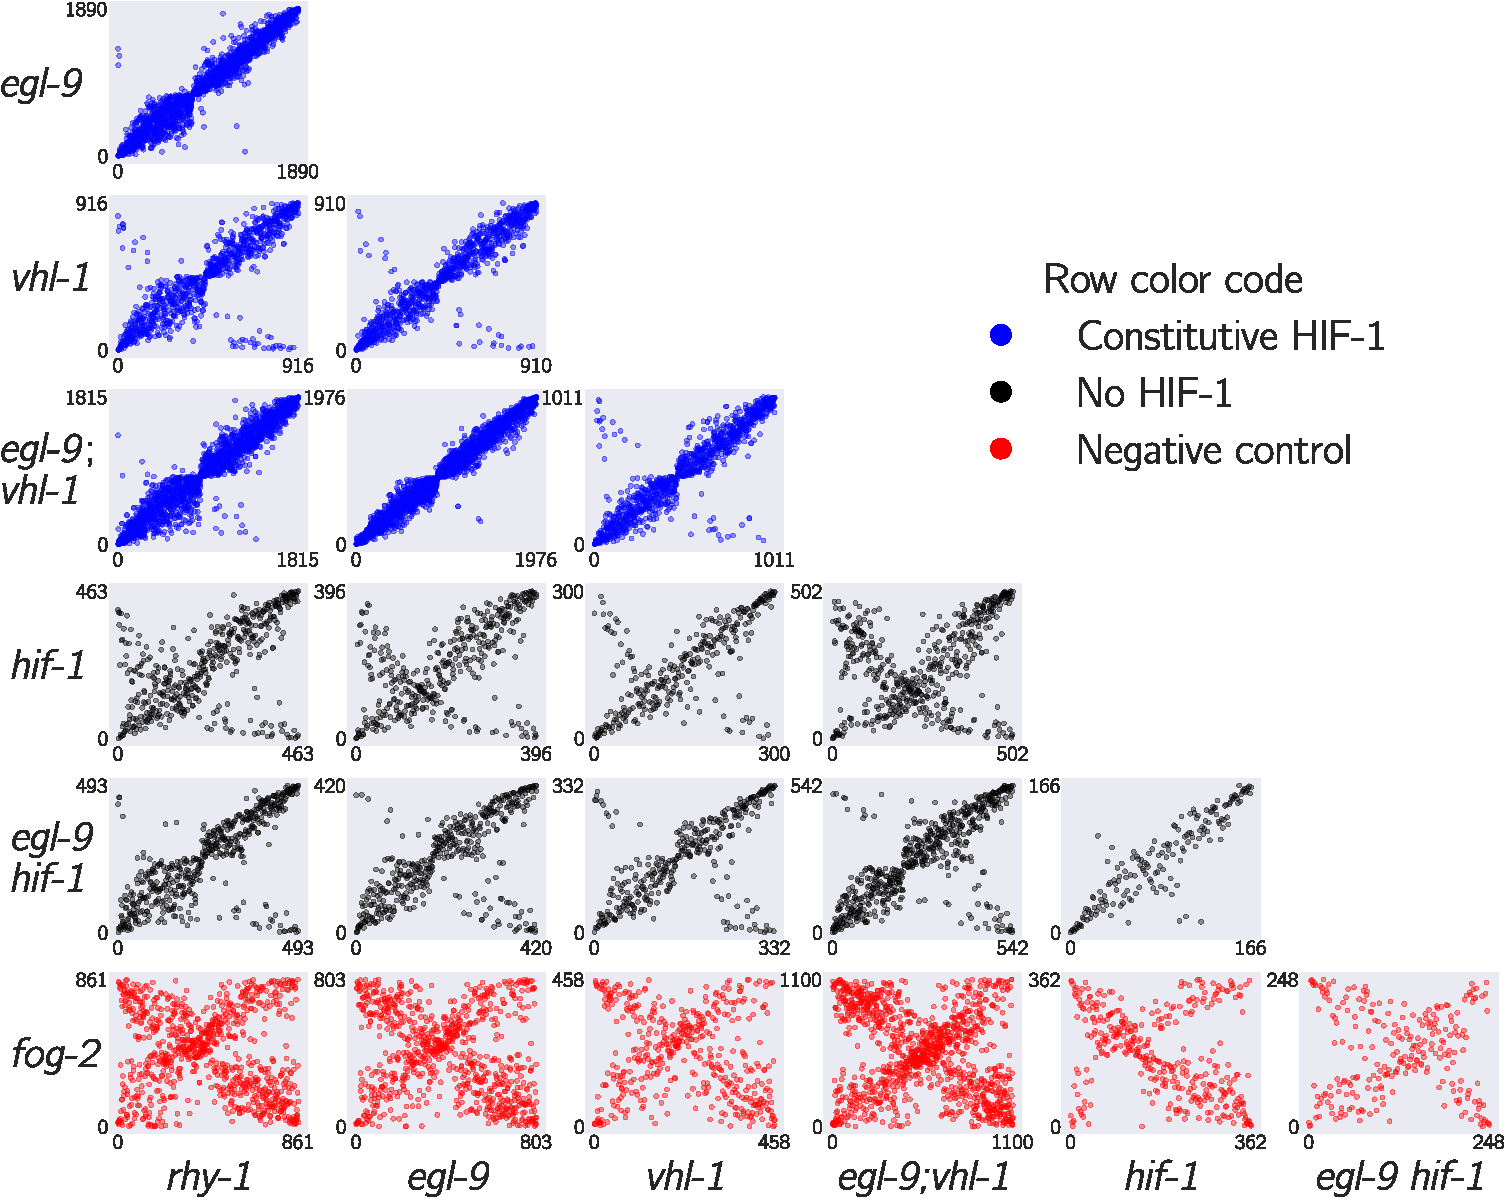
\includegraphics[width=\textwidth]{hypims/triangle_plot.pdf}
  \caption{
  Interacting genes have correlated transcriptional signatures. The rank order
  of transcripts contained in the shared transcriptional phenotype is plotted
  for each pairwise combination of genotypes.Correlations between in-pathway
  genotypes are strong whereas comparisons with a \fog{} genotype are dominated
  by noise. Comparisons between some genotypes show populations of transcripts
  that are anticorrelated, possibly as a result of feedback loops. Plots are
  color-coded by row. Comparisons with genotypes with a constitutive hypoxia
  response are in blue; comparisons with genotypes negative for \hif{} are
  black; and comparisons involving \fog{} are red. X- and y-axes show the rank
  of each transcript within each genotype.
  }
\label{fig:genetic_interactions}
\end{figure}

Next, we analyzed pairwise correlations between all mutant pairs. We
rank-transformed the $\beta$ coefficients of each isoform between the STP of two
mutants, and plotted the transcript ranks between genotypes (see
Fig~\ref{fig:genetic_interactions}).
% For mutants
% associated with the hypoxia pathway, these correlations have values higher than
% 0.9 with a tight distribution around the line of best fit.
% The correlations for
% mutants from the hypoxia pathway with the \fog{} mutant were considerably
% weaker, with magnitudes between 0.6--0.85 and greater variance around the line
% of best fit.
Although \gene{hif-1} is known to be genetically repressed by
\gene{egl-9}, \gene{rhy-1} and \gene{vhl-1}~\citep{Epstein2001,Shen2006}, all the
correlations between mutants of these genes and \hif{} were positive (see
\href{https://wormlabcaltech.github.io/mprsq/analysis_notebooks/2_predict_interactions.html}
{Genetic Interactions Notebook}). We reasoned that this apparent contradiction
could be due to either strain-specific effects in our N2 background (an
artifactual signal) or that it could reflect a previously unrecognized aspect of
\hifp{} biology. This motivated us to look for genes that exhibited verifiable
extreme patterns of anomalous behavior and led us to propose a new model of the
hypoxia pathway (see Identification of non-classical epistatic interactions).

\subsection*{Transcriptome-wide epistasis}
Ideally, any measurement of transcriptome-wide epistasis should conform to
certain expectations. First, it should make use of the regression coefficients
of as many genes as possible. Second, it should be summarizable in a single,
well-defined number. Third, it should have an intuitive behavior, such that
special values of the statistic have an unambiguous interpretation.

We found an approach that satisfies all of the above conditions and which can be
graphed in an epistasis plot (see Fig~\ref{fig:egl9epistasis}) In an epistasis
plot, the X-axis represents the expected $\beta$ coefficient for given gene in a
double mutant $a^-b^-$ if $a$ and $b$ interact log-additively. In other words,
each individual isoform's x-coordinate is the sum of the regression coefficients
from the single mutants $a^-$ and $b^-$. The Y-axis represents the deviations
from the log-additive (null) model, and can be calculated as the difference
between the predicted and the observed $\beta$ coefficients. Only isoforms that
are differentially expressed in all three genotypes are plotted. This attempts
to ensure that the isoforms to be examined are regulated by both genes. These
plots will generate specific patterns that can be described through linear
regressions. The slope of these lines, to which we assign the mathematical
notation $s({a,b})$, is the transcriptome-wide epistasis coefficient.
Importantly, the transcriptome-wide epistasis coefficient is fundamentally
distinct from  Pearson or Spearman correlation coefficients and need not have a
simple linear mapping. In other words, negative correlation coefficients do not
imply a specific sign of the epistasis coefficient, and \emph{vice versa}. For
suppression to occur, for example, the only requirement is that the phenotype of
the double mutant should match one, and only one, of the two single mutants. The
value of the correlation coefficient is not relevant.

Transcriptome-wide epistasis coefficients can be understood intuitively for
simple cases of genetic interactions if complete genetic nulls are used. If two
genes act additively on the same set of differentially expressed isoforms then
all the plotted points will fall along the line $y=0$. If two genes act
positively in an unbranched pathway, then all the mutants should have the same
phenotype. It follows that data from this pathway will form line with slope
equal to $-\frac{1}{2}$. On the other hand, in the limit of complete genetic
inhibition of $b$ by $a$ in an unbranched pathway (i.e., $a$ is in great excess
over $b$, such that under the conditions measured $b$ has no activity), the
plots should show a line of best fit with slope equal to $-1$. Genes that
interact synthetically (\emph{i.e.}, through an OR-gate) will fall along lines
with slopes $>0$. When there is epistasis of one gene over another, the points
will fall along one of two possible slopes that must be determined empirically
from the single mutant data. We can use both single mutant data to predict the
distribution of slopes that results for the cases stated above. Thus, the
transcriptome-wide epistasis coefficient integrates information from many
different isoforms into a single number (see Fig.~\ref{fig:egl9epistasis}).

In our experiment, we studied two double mutants, \eglhif{} and \eglvhl{}. We
wanted to understand how well an epistatic analysis based on transcriptome-wide
coefficients agreed with the epistasis results reported in the literature, which
were based on qPCR of single genes. Therefore, we determined the epistasis
coefficient of the two gene combinations we studied (\gene{egl-9} and
\gene{vhl-1}, and \gene{egl-9} and \gene{hif-1}). In addition to computing an
epistasis coefficient from these factors, we would like to know which gene is
suppressed in the double mutant. Suppression means that the double mutant
should have exactly the phenotype of one and only one mutant, we can simulate
the double mutant by replacing the double mutant data with either of the two
single mutants and matching the simulated result to the observed result. The
result that most closely matches the real data will reveal which gene is being
suppressed, which in turn allows us to order the genes along a pathway.

We measured the epistasis coefficient between \gene{egl-9} and \gene{vhl-1},
$s({\text{\gene{egl-9} \gene{vhl-1}}}) = -0.41\pm 0.01$ (see
\href{https://wormlabcaltech.github.io/mprsq/analysis_notebooks/6_epistasis.html}
{Epistasis Notebook}). Simulations using just the single mutant data showed that
the double mutant exhibited the \egl{} phenotype (see
Fig.~\ref{fig:egl9epistasis}). We used Bayesian model selection to reject a
linear pathway (odds ratio (OR) $>10^{92}$), which leads us to conclude
\gene{egl-9} is upstream of \gene{vhl-1} acting on a phenotype in a branched
manner. We also measured epistasis between \gene{egl-9} and \gene{hif-1},
$s({\text{\gene{egl-9}, \gene{hif-1}}}) = -0.80\pm0.01$ (see SI Figure 2), and
we found that this behavior could be predicted by modeling \gene{hif-1}
downstream of \gene{egl-9}. We also rejected the null hypothesis that these two
genes act in a positive linear pathway (OR$> 10^{93}$). Taken together, this
leads us to conclude that \gene{egl-9} strongly inhibits \gene{hif-1}.

% epistasis graph
\begin{figure}[tbhp]
  \centering
  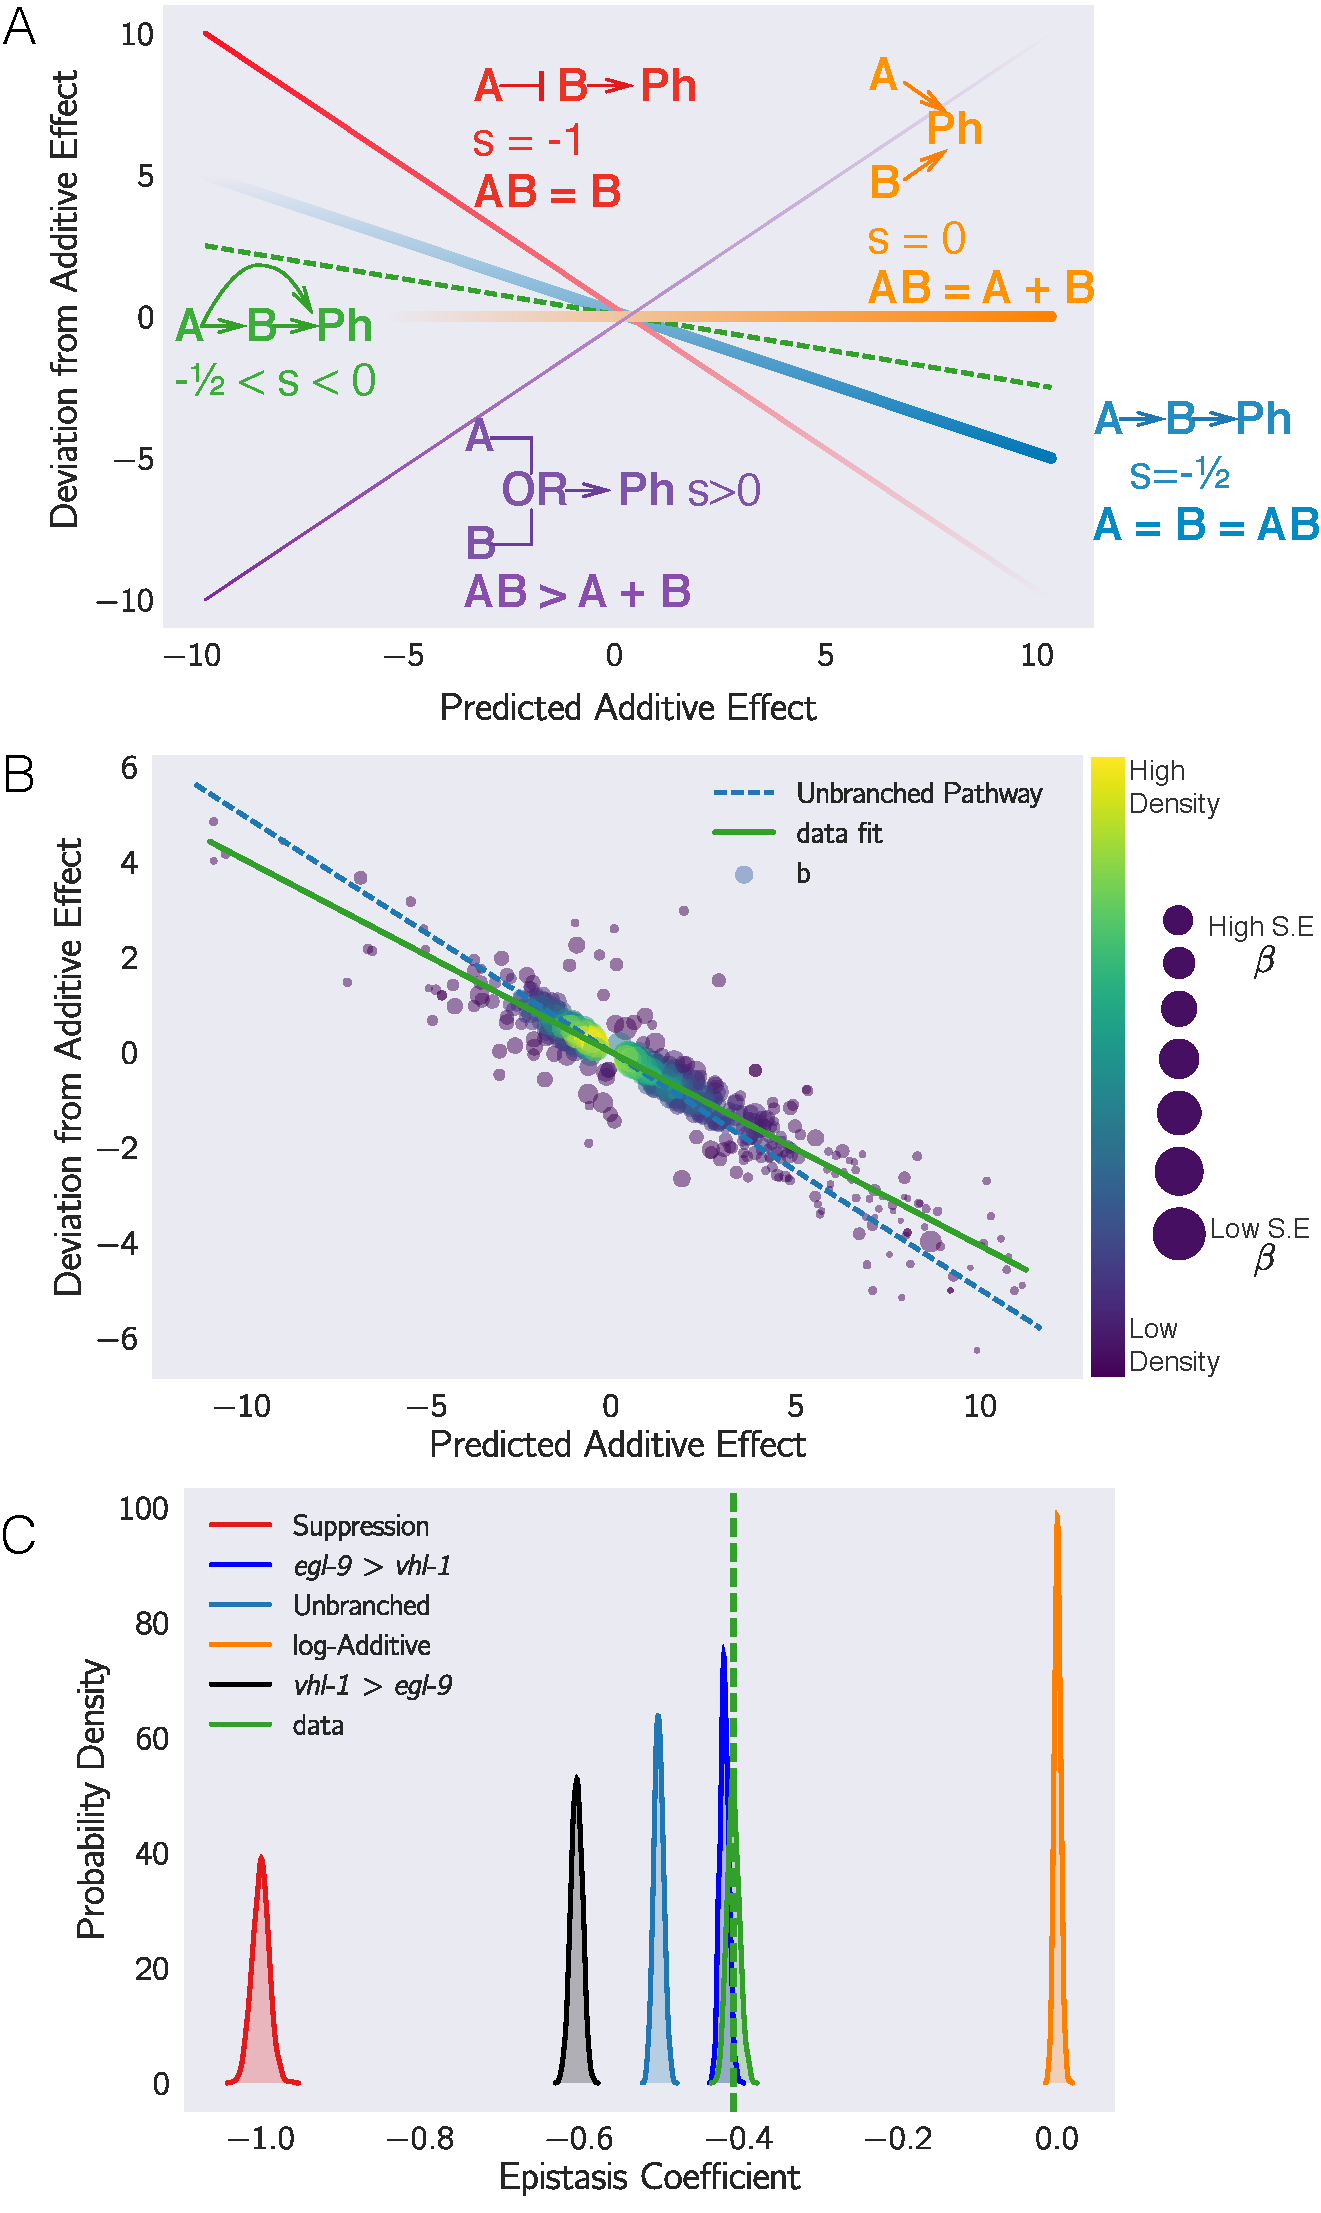
\includegraphics[width=.5\textwidth]{hypims/egl9vhl1-epistasis.pdf}
  \caption{
    (\textbf{A}) Schematic diagram of an epistasis plot. The X-axis on an
    epistasis plot is the expected coefficient for a double mutant under an
    log-additive model (null model). The Y-axis plots deviations from this
    model. Double mutants that deviate in a systematic manner from the null
    model exhibit transcriptome-wide epistasis ($s$). To measure $s$, we find
    the line of best fit and determine its slope. Genes that act log-additively
    on a phenotype \textbf{(Ph)} will have $s=0$ (null hypothesis, orange line);
    whereas genes that act along an unbranched pathway will have $s=-1/2$ (blue
    line). Strong repression is reflected by $s=-1$ (red line), whereas $s>0$
    correspond to synthetic interactions (purple line). (\textbf{B}) Epistasis
    plot showing that the \eglvhl{} transcriptome deviates significantly from a
    null additive. Points are colored qualitatively according to density
    (purple---low, yellow---high) and size is inversely proportional to the
    standard error (S.E.) of the y-axis. The green line is the line of best fit
    from an orthogonal distance regression. (\textbf{C}) Comparison of simulated
    epistatic coefficients against the observed coefficient. Green curve shows
    the bootstrapped observed transcriptome-wide epistasis coefficient for
    \gene{egl-9} and \gene{vhl-1}. Dashed green line shows the mean value of the
    data. Simulations use only the single mutant data to idealize what
    expression of the double mutant should look like. $a > b$ means that the
    phenotype of $a$ is observed in a double mutant $a^-b^-$. }
\label{fig:egl9epistasis}
\end{figure}

\subsubsection*{Epistasis between two genes can be predicted using an upstream component}
Given our success in measuring epistasis coefficients, we wanted to know whether
it would be possible to predict the epistasis coefficient between \gene{egl-9}
and \gene{vhl-1} in the absence of the \egl{} genotype. Since \rhyp{} indirectly
activates \eglp{}, we reasoned that the \rhy{} transcriptome should contain
almost equivalent information to the \egl{} transcriptome. Therefore, we
generated predictions of the epistasis coefficient between \gene{egl-9} and
\gene{vhl-1} by substituting in the \rhy{} data, predicting $s({rhy-1,vhl-1}) =
-0.45$. Similarly, we used the \eglvhl{} double mutant to measure the epistasis
coefficient while replacing the \egl{} dataset with the \rhy{} dataset. We found
that the epistasis coefficient using this substitution was $-0.38\pm 0.01$. This
coefficient was different from $-0.50$ (OR $>10^{102}$), reflecting the same
qualitative conclusion that \gene{vhl-1} represents a branch in the hypoxia
pathway. We were able to obtain a close prediction of the epistasis coefficient
for two mutants using the transcriptome of a related, upstream mutant.

\subsection*{Transcriptomic decorrelation can be used to infer functional distance}
\label{sub:decorrelation}
% What are functional interactions?
So far, we have shown that RNA-seq can accurately measure genetic interactions.
However, genetic interactions do not require two gene products to interact
biochemically, nor even to be physically close to each other. RNA-seq cannot
measure physical interactions between genes, but we wondered whether expression
profiling contains sufficient information to order genes along a pathway.

Single genes are often regulated by multiple independent sources. The connection
between two nodes can in theory be characterized by the strength of the edges
connecting them (the thickness of the edge); the sources that regulate both
nodes (the fraction of inputs common to both nodes); and the genes that are
regulated by both nodes (the fraction of outputs that are common to both nodes).
In other words, we expected that expression profiles associated with a pathway
would respond quantitatively to quantitative changes in activity of the pathway.
Targeting a pathway at multiple points would lead to expression profile
divergence as we compare nodes that are separated by more degrees of freedom,
reflecting the flux in information between them.

% decorrelation
\begin{figure}[tbhp]
  \centering
  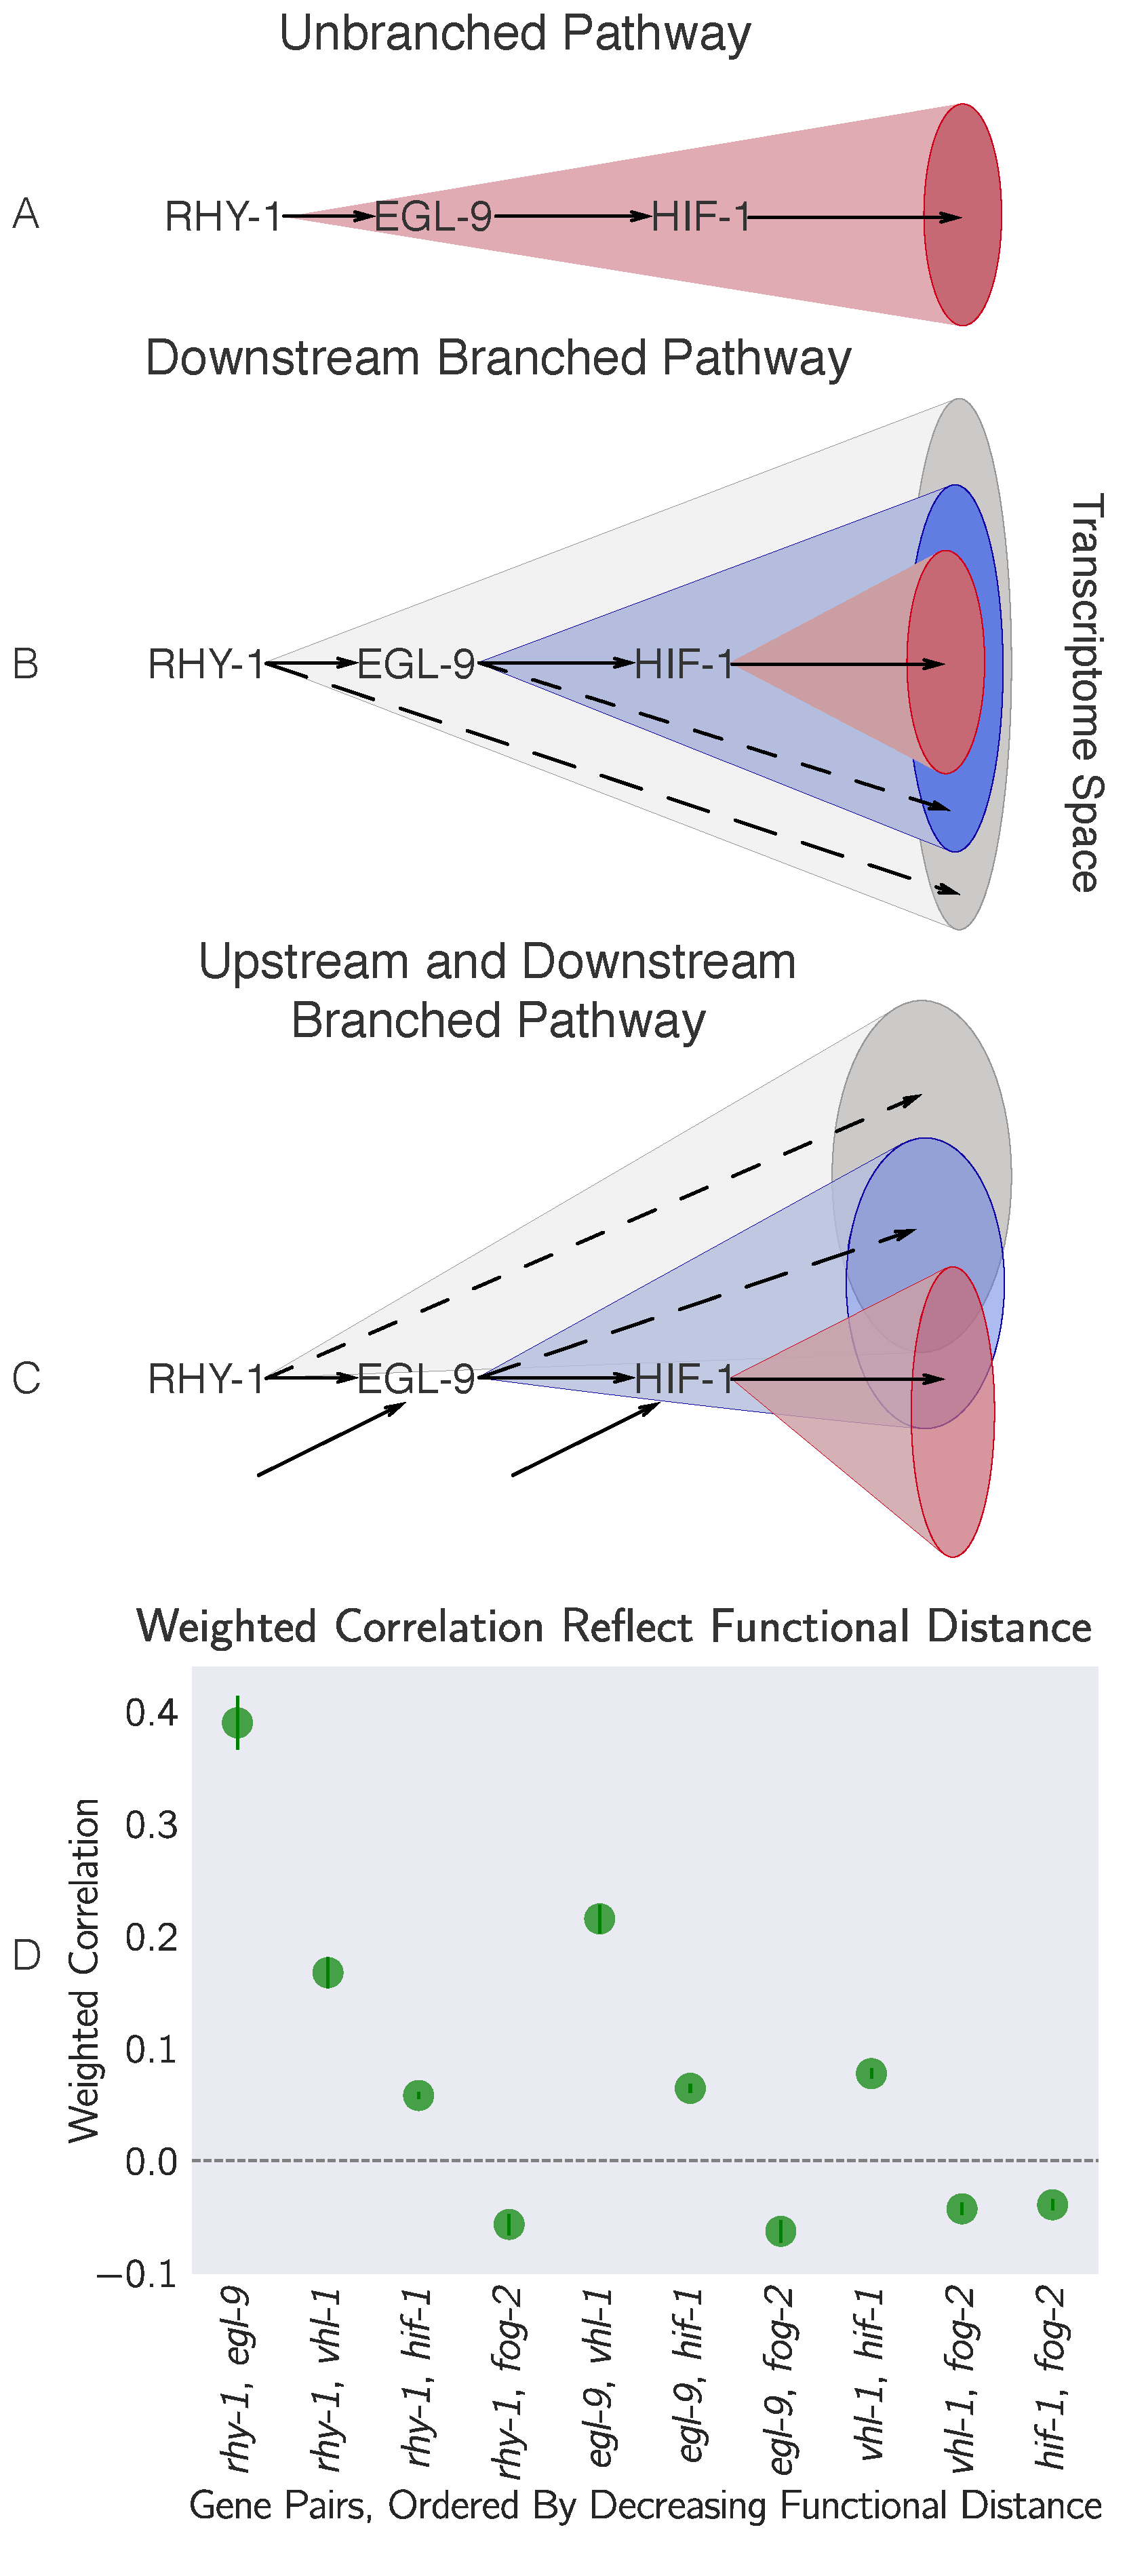
\includegraphics[width=.4\textwidth]{hypims/decorrelation.pdf}
  \caption{
    Transcriptomes can be used to order genes in a pathway under
    certain assumptions. Arrows in the diagrams above are intended to show the
    direction of flow, and do not indicate valence. \textbf{A}. A linear pathway
    in which \gene{rhy-1} is the only gene controlling \gene{egl-9}, which in
    turn controls \gene{hif-1} does not contain information to infer the order
    between genes. \textbf{B}. If \gene{rhy-1} and \gene{egl-9} have
    transcriptomic effects that are separable from \gene{hif-1}, then the
    \gene{rhy-1} transcriptome should contain contributions from \gene{egl-9},
    \gene{hif-1} and \gene{egl-9}- and \gene{hif-1}-independent pathways. This
    pathway contains enough information to infer order. \textbf{C}. If a pathway
    is branched both upstream and downstream, transcriptomes will show even
    faster decorrelation. Nodes that are separated by many edges may begin to
    behave almost independently of each other with marginal transcriptomic
    overlap or correlation. \textbf{D}. The hypoxia pathway can be ordered. We
    hypothesize the rapid decay in correlation is due to a mixture of upstream
    and downstream branching that happens along this pathway. Bars show the
    standard error of the weighted coefficient from the Monte Carlo Markov Chain
    computations.
  }
\label{fig:decorrelation}
\end{figure}

We investigated this possibility by weighting the robust Bayesian regression
between each pair of genotypes by the size of the shared transcriptomic
phenotype of each pair divided by the total number of isoforms differentially
expressed in either mutant ($N_\mathrm{Intersection}/N_{\mathrm{Union}}$). We
plotted the weighted correlation of each gene pair, ordered by increasing
functional distance (see Fig.~\ref{fig:decorrelation}). In every case, we see
that the weighted correlation decreases monotonically due mainly, but not
exclusively, to a smaller STP (see
\href{https://wormlabcaltech.github.io/mprsq/analysis_notebooks/10_decorrelation.html}
{Decorrelation Notebook}).

We believe that this result is not due to random noise or insufficiently deep
sequencing. Instead, we propose a framework in which every gene is regulated by
multiple different molecular species, which induces progressive decorrelation.
This decorrelation in turn has two consequences. First, decorrelation within a
pathway implies that two nodes may be almost independent of each other if the
functional distance between them is large. Second, it may be possible to use
decorrelation dynamics to infer gene order in a branching pathway, as we have
done with the hypoxia pathway.

\subsection*{Classical epistasis identifies a core hypoxic response}
We searched for genes whose expression obeyed the two epistatic equality
relationships, \hif{}=\eglhif{} and \egl{}=\eglvhl{}, since these equalities
define the hypoxia pathway. We excluded genes whose expression deviated from
this relationship by more than 2 standard deviations or that had opposite
changes in direction. Using these criteria, we identified 1,258 genes in the
hypoxia response. Tissue Enrichment Analysis showed that the intestine and
epithelial system were enriched in this response (\qval{10} for both terms),
consistent with previous reports~\citep{Budde2010}. Gene Enrichment
Analysis~\citep{Angeles-Albores106369} showed enrichment in the mitochondrion and
in collagen trimers (\qval{10}) (see
\href{https://wormlabcaltech.github.io/mprsq/analysis_notebooks/3_ea_of_hypoxia_data.html}
{Enrichment Analysis Notebook} and SI Figures 3 and 4). This response included
15 transcription factors. Even though \hifp{} is
an activator, not all of these genes were up-regulated. We reasoned that only
genes that are up-regulated in \hifp{}-inhibitor mutants are candidates for
direct regulation by \hifp{}. We found \hiftargets{} such genes.

\subsection*{Feedback can be inferred}
\label{sub:topology}
While some of the rank plots contained a clear positive correlation, others
showed a discernible cross-pattern (see Fig.~\ref{fig:genetic_interactions}). In
particular, this cross-pattern emerged between \vhl{} and \rhy{} or between
\vhl{} and \egl{}, even though \gene{vhl-1}, \gene{rhy-1} and \gene{egl-9} are
all inhibitors of \hif{}. Such cross-patterns could be indicative of feedback
loops or other complex interaction patterns. If the above is correct, then it
should be possible to identify genes that are regulated by \gene{rhy-1} in a
logically consistent way: Since loss of \gene{egl-9} causes \gene{rhy-1} mRNA
levels to increase, if this increase leads to a significant change in RHY-1
activity, then it follows that the \egl{} and \rhy{} should show
anti-correlation in a subset of genes. Since we do not observe many genes that
are anti-correlated, we conclude that is unlikely that the change in
\gene{rhy-1} mRNA expression causes a significant change in RHY-1 activity under
normoxic conditions. We also searched for genes with \gene{hif-1}-independent,
\gene{vhl-1}-dependent gene expression and found \vhltargets{} genes (SI File
1).



\subsection*{Identification of non-classical epistatic interactions}
\label{sub:hifoh}
\hif{} has traditionally been viewed as existing in a genetic OFF state under
normoxic conditions. However, our dataset indicates that \hifn{} genes show
altered expression when \gene{hif-1} function is removed in normoxic conditions.
Moreover, we observed positive correlations between \hif{} $\beta$ coefficients
and \egl{}, \vhl{} and \rhy{} $\beta$ coefficients in spite of the negative
regulatory relationships between these genes and \gene{hif-1}. Such positive
correlations could indicate a relationship between these genes that has not
been reported previously.

We identified genes that exhibited violations of the canonical genetic
model of the hypoxia pathway (see Fig.~\ref{fig:hif1oh}; also
\href{https://wormlabcaltech.github.io/mprsq/analysis_notebooks/7_hifoh.html}
{Non-canonical epistasis notebook}). We searched for genes that changed in different
directions between \egl{} and \vhl{}, or, equivalently, between \rhy{} and
\vhl{} (we assume that all results from the \rhy{} transcriptome reflect a
complete loss of \gene{egl-9} activity) without specifying any further
conditions. We found \hifohtargets{} that satisfied this condition (see
Fig.~\ref{fig:hif1oh}, SI File 1). When we checked expression of
these genes in the double mutant, we found that \gene{egl-9} remained epistatic
over \gene{vhl-1} for this class of genes. This class of genes may in fact be
larger because it overlooks genes that have wild-type expression in an
\egl{} background, altered expression in a \vhl{} background, and suppressed
(wild-type) expression  in an \eglvhl{} background.
As a result, it could help
explain why the \hif{} mutant transcriptome is positively correlated with its
inhibitors.

\begin{figure}[tbhp]
  \centering
  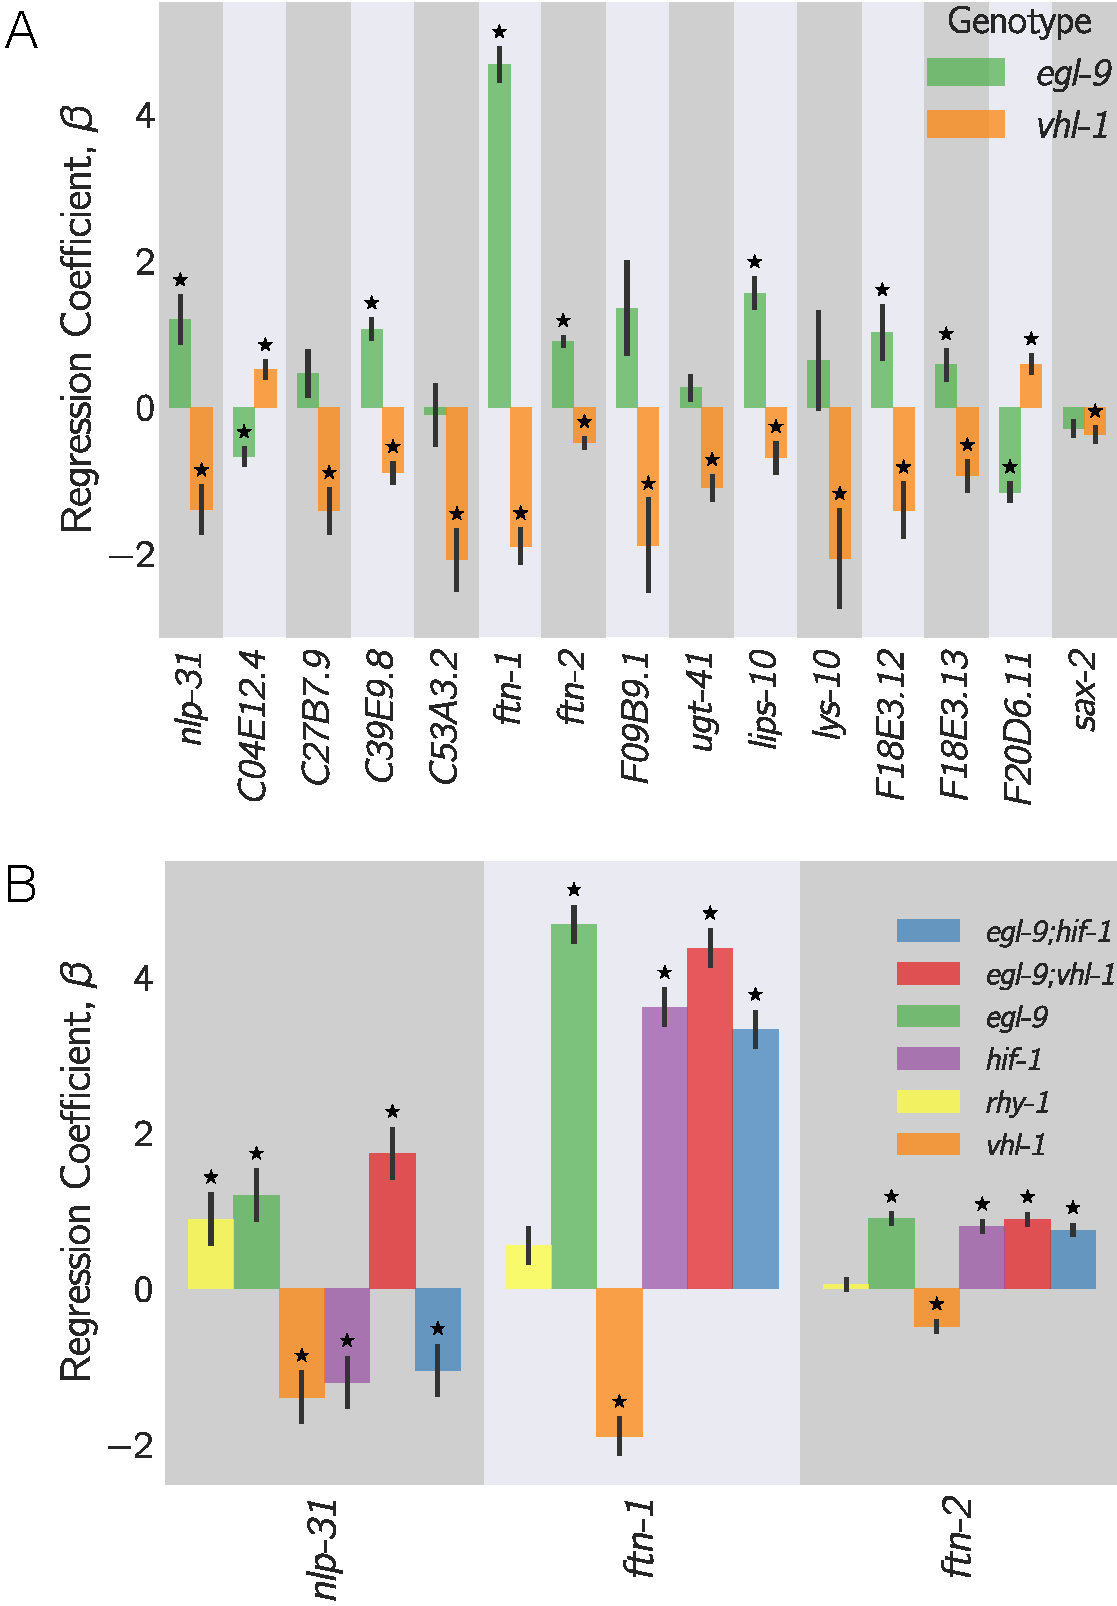
\includegraphics[width=.5\textwidth]{hypims/hif1oh_epistasis.pdf}
  \caption{
    \textbf{A}. \hifohtargets{} genes in \cel{} exhibit non-classical epistasis
    in the hypoxia pathway, characterized by opposite effects on gene expression,
    relative to the wild type, of the \vhl{} compared to \egl{} (or \rhy{})
    mutants. Shown are a random selection of 15 out of \hifohtargets{} genes for
    illustrative purposes. \textbf{B}. Genes that behave non-canonically  have a
    consistent pattern. \vhl{} mutants have an opposite effect to \egl{}, but
    \gene{egl-9} remains epistatic to \gene{vhl-1} and loss-of-function
    mutations in \gene{hif-1} suppress the \egl{} phenotype. Asterisks show
    $\beta$ values significantly different from 0 relative to wild type
    (\qval{1}).
  }
\label{fig:hif1oh}
\end{figure}

Although this entire class had similar behavior, we focused on two genes, \nlp{}
and \ftna{} which have representative expression patterns. \ftna{} is described
to be responsive to mutations in the hypoxia pathway and has been reported to
have aberrant behaviors; specifically, loss of function of \gene{egl-9} and
\gene{vhl-1} have opposing effects on \ftna{}
expression~\citep{Ackerman2012,Romney2011}. These studies showed the same \ftna{}
expression phenotypes using RNAi and alleles, allaying concerns of
strain-specific interference. We observed that \gene{hif-1} was epistatic to
\gene{egl-9}, and that \gene{egl-9} and \gene{hif-1} both promoted \ftna{}
expression.

Analysis of \ftna{} expression reveals that \gene{egl-9} is epistatic to
\gene{hif-1}; that \gene{vhl-1} has opposite effects to \gene{egl-9}, and that
\gene{vhl-1} is epistatic to \gene{egl-9}. Analysis of \nlp{} reveals similar
relationships. \nlp{} expression is decreased in \hif{}, and increased in
\egl{}. However, \gene{egl-9} is epistatic to \gene{hif-1}. Like \ftna{},
\gene{vhl-1} has the opposite effect to \gene{egl-9}, yet is epistatic to
\gene{egl-9}. We propose in the Discussion a novel model for how \hifp{} might
regulate these targets.


\section*{Discussion}
\label{sec:hyp_discussion}
\subsection*{The \cel{} hypoxia pathway can be reconstructed \emph{de novo} from
             RNA-seq data}
We have shown that whole-organism transcriptomic phenotypes can
be used to reconstruct genetic pathways and to discern previously
uncharacterized genetic interactions. We successfully reconstructed the hypoxia
pathway including the order of action of the genetic components and its
branching pattern.
These results highlight the potential of whole-animal
expression profiles for dissecting molecular pathways that are expressed in a
large number of cells within an organism. While our results are promising, it
remains to be seen whether our approach will also work for pathways that act in
a few cells. We selected a previously characterized pathway because \cel{} is
less amenable to high-throughput screens compared to cultured cells. That said,
the striking nature of our results makes us optimistic that this technique could
be successfully used to reconstruct unknown pathways.

\subsection*{Interpretation of the non-classical epistasis in the hypoxia pathway}
The \hifohtargets{} genes that exhibit a striking pattern of
non-classical epistasis suggest the existence of previously undescribed aspects
of the hypoxia pathway. Some of these non-classical behaviors had been observed
previously~\citep{Ackerman2012,Romney2011,Luhachack2012}, but no satisfactory
mechanism has been proposed to explain them. Previous
studies~\citep{Romney2011,Ackerman2012} suggested that \hifp{} integrates
information on iron concentration in the cell to determine its binding affinity
to the \ftna{} promoter, but could not definitively establish a mechanism. It is
unclear why deletion of \gene{hif-1} and deletion of \gene{egl-9} both cause
induction of \ftna{} expression, but deletion of \gene{vhl-1} abolishes this
induction. Moreover, Luchachack et al~\citep{Luhachack2012} have previously
reported that certain genes important for the \cel{} immune response against
pathogens reflect similar non-canonical expression patterns. Their
interpretation was that \gene{swan-1}, which encodes a binding partner to
\eglp{}~\citep{Shao2010}, is important for modulating \hifp{} activity in some
manner. The lack of a conclusive double mutant analysis in this work means the
role of SWAN-1 in modulation of \hifp{} activity remains to be demonstrated.
Other mechanisms, such as tissue-specific differences in the
pathway~\citep{Budde2010} could also modulate expression, though it is worth
pointing out that \ftna{} expression appears restricted to a single tissue, the
intestine~\citep{Kim2004}. Another possibility is that \gene{egl-9} controls
\gene{hif-1} mRNA stability via other \gene{vhl-1}-independent pathways, but we
did not see a decreases in \gene{hif-1} level in \egl{}, \rhy{} or \vhl{} mutants.
Another possibility, such as control of protein stability via \gene{egl-9}
independently of \gene{vhl-1}~\citep{Chintala2012} will not lead to splitting
unless it happens in a tissue-specific manner.

\begin{figure}[tbhp]
  \centering
  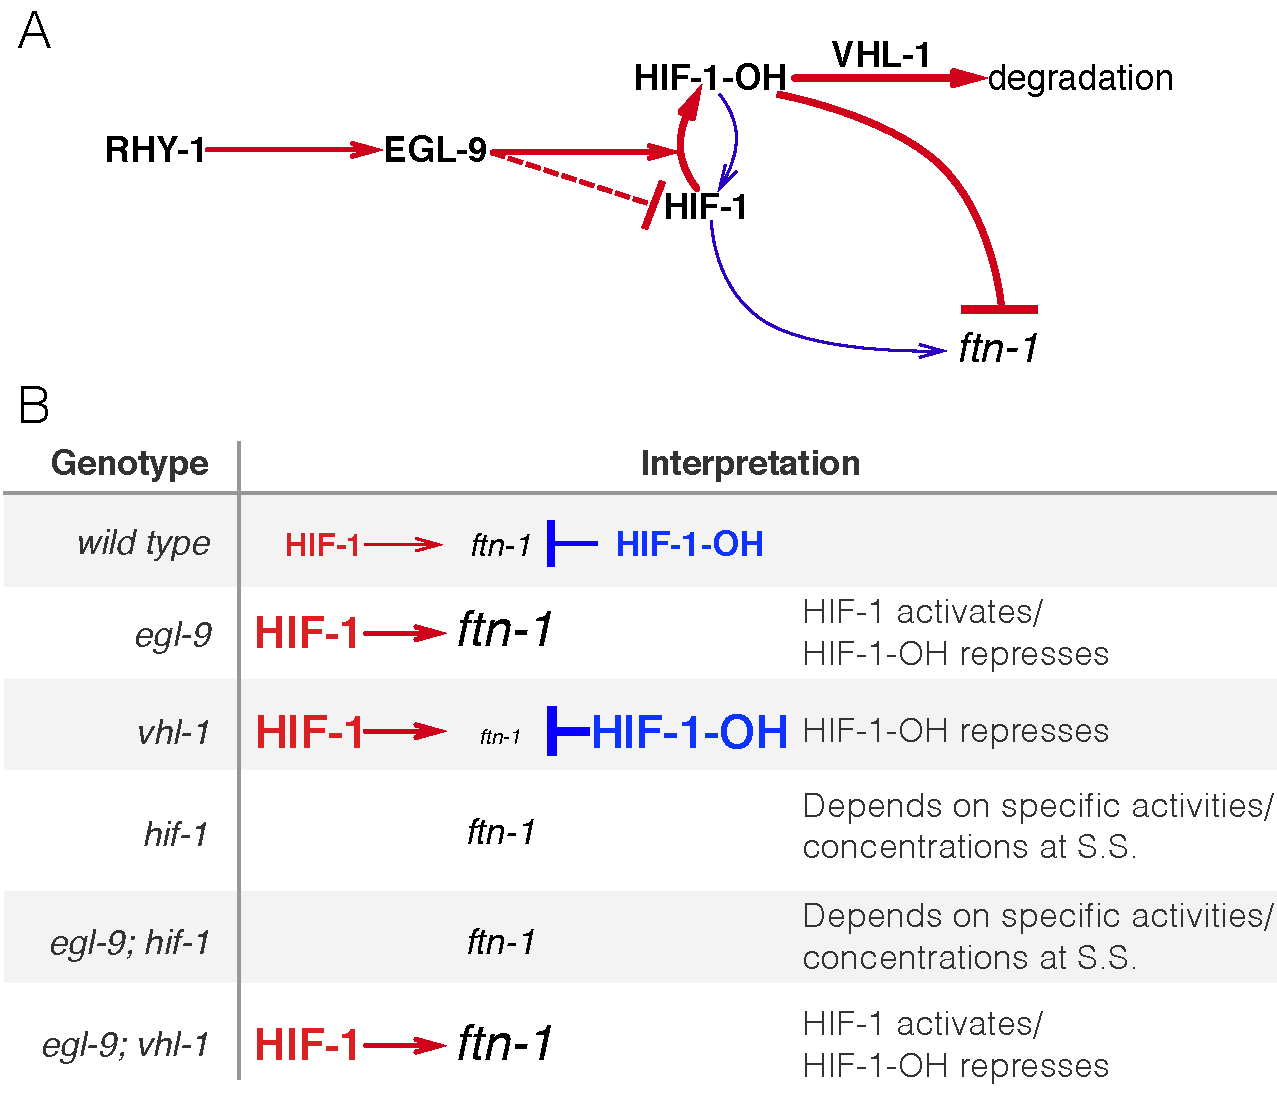
\includegraphics[width=\textwidth]{hypims/hif1oh_model.pdf}
  \caption{
    A hypothetical model showing a mechanism where \hifp{}-hydroxyl antagonizes
    \hifp{} in normoxia. \textbf{A}. Diagram showing that RHY-1 activates EGL-9.
    EGL-9 hydroxylates HIF-1 in an oxygen-dependent manner. HIF-1 is
    rapidly hydroxylated and the product, HIF-1-OH is rapidly degraded in a
    VHL-1-dependent fashion. EGL-9 can also inhibit
    HIF-1 in an oxygen-independent fashion. In our model, HIF-1 and HIF-1-OH
    have opposing effects on transcription. The width of the arrows represents
    rates in normoxic conditions.
    \textbf{B}. Table showing the effects of loss-of-function mutations on HIF-1
    and HIF-1-OH activity, showing how this can potentially explain the
    \gene{ftn-1} expression levels in each case. S.S = Steady-state.
  }
\label{fig:hif1oh_table}
\end{figure}

One parsimonious solution is to consider \hifp{} as a protein with both
activating and inhibiting states. In fact, \hifp{} already exists in two states
in \cel{}: unmodified \hifp{} and \hifp{}-hydroxyl (\hifp{}-OH). Under this
model, the effects of \hifp{} for certain genes like \ftna{} or \nlp{} are
antagonized by \hifp{}-hydroxyl, which is present at only a low level in the
cell in normoxia because it is degraded in a \gene{vhl-1}-dependent fashion.
This means that loss of \gene{vhl-1} stabilizes \hifp{}-hydroxyl. If \gene{vhl-1}
is inactivated, genes that are
sensitive to \hifp{}-hydroxyl will be inhibited as a result of the increase in
\hifp{}-hydroxyl, despite the increased levels of
non-hydroxylated \hifp{}. On the other hand, \egl{}
abrogates the generation of \hifp{}-hydroxyl, stimulating accumulation of
non-hydroxylated \hifp{} and promoting gene expression. Whether deletion of \hif{}
is overall activating or inhibiting will depend on the relative activity of each
protein state under normoxia (see Fig.~\ref{fig:hif1oh_table}). \hifp{}-hydroxyl
is challenging to study genetically, and if it does have the activity suggested
by our genetic evidence this may have prevented such a role from being detected.
No mimetic mutations are known with which to study the pure
hydroxylated \hifp{} species, and mutations in the Von Hippel-Lindau gene that
stabilize the hydroxyl species also increase the quantity of non-hydroxylated
\hifp{} by mass action.

Because \hifp{} is detected at low levels in cells under normoxic
conditions~\citep{Wang1993}, total \hifp{} protein levels are assumed to be so
low as to be biologically inactive. However, our data show \hifn{} genes change
expression in response to loss of \gene{hif-1} under normoxic conditions, which
establishes that there is sufficient total \hifp{} protein to be biologically
active. Our analyses also revealed that \hif{} shares positive correlations with
\egl{}, \rhy{} and \vhl{}, and that each of these genotypes also shows a
secondary negative rank-ordered expression correlation with each other.

% These
% cross-patterns between all loss of function of inhibitors of \hifp{} and \hif{}
% can be most easily explained if \hifp{}-hydroxyl is biologically active.

A homeostatic argument can be made in favor of the activity of \hifp{}-hydroxyl.
The cell must continuously monitor multiple metabolite levels. The
\gene{hif-1}-dependent hypoxia response integrates information from O$_2$,
$\alpha$-ketoglutarate and iron concentrations in the cell. One
way to integrate this information is by encoding it within the effective
hydroxylation rate of \hifp{} by \eglp{}. Then the dynamics in this system will
evolve exclusively as a result of the total amount of \hifp{} in the cell. Such
a system can be sensitive to fluctuations in the absolute concentration of
\hifp{}~\citep{Goentoro2009a}. Since the absolute levels of \hifp{} are low in
normoxic conditions, small fluctuations in protein copy-number can represent a
large fold-change in \hifp{} levels. These fluctuations might not be problematic
for genes that must be turned on only under conditions of severe
hypoxia---presumably, these genes would be activated only when \hifp{} levels
increase far beyond random fluctuations.

For yet other sets of genes that must change expression in response to the
hypoxia pathway, it may not be sufficient to integrate metabolite
information exclusively via \eglp{}-dependent hydroxylation of \hifp{}. In
particular, genes that may function to increase survival in mild hypoxia may
benefit from regulatory mechanisms that can sense minor changes in environmental
conditions and which therefore benefit from robustness to transient changes in
protein copy number. Likewise, genes that are involved in iron or
$\alpha$-ketoglutarate metabolism (such as \ftna{}) may benefit from being able
to sense, accurately, small and consistent deviations from basal concentrations
of these metabolites. For these genes, the information may be better encoded by
using \hifp{} and \hifp{}-hydroxyl as an activator/repressor pair. Such circuits
are known to possess distinct advantages for controlling output robustly to
transient fluctuations in the levels of their
components~\citep{Hart2012,Hart2013}.

Our RNA-seq data suggests that one of these atypical targets of \hifp{} may be
\rhyp{}. Although \gene{rhy-1} does not exhibit non-classical epistasis, all
genotypes containing a \hif{} mutation had increased expression levels of
\gene{rhy-1}. We speculate that if \gene{rhy-1} is controlled by both \hifp{}
and \hifp{}-hydroxyl, then this might imply that \hifp{} auto-regulates both
positively and negatively.

\subsection*{Strengths and weaknesses of the methodology}
We have described a set of methods that can in principle be applied to
any multidimensional phenotype. Although we have not applied these methods to
\emph{de novo} pathway discovery, we believe that they will be broadly
applicable to a wide variety of genetic problems. One aspect of our methodology
is the use of whole-organism expression data. Data collection from
whole-organisms can be rapid with low technical barriers. On the other
hand, a concern is that whole-organism data will average signals across tissues,
which would limit the scope of this technology to the study of genetic pathways
that are systemic or expressed in large tissues. In
reality, our method may be applicable for pathways that are expressed even in a
small number of cells in an organism. If a pathway is active in a single cell,
this does not mean that it does not have cell-non-autonomous effects that could
be detected on an organism-wide level. Thus,
pathways that act in single cells could still be
characterized via whole-organism transcriptome profiling. If the non-autonomous
effects are long-lasting, then the profiling could take place after the
time-of-action of this pathway. In fact, this is how the female-like state in
\cel{} was recently identified~\citep{Angeles-Albores2017}: \gene{fog-2} is
involved in translation repression of \gene{tra-2} in the somatic gonad,
thereby promoting sperm formation in late larvae~\citep{Clifford2000}.
Loss of this gene causes non-cell-autonomous effects that can be detected well
after the time-of-action of \gene{fog-2} in the somatic gonad has ended.
Therefore, we believe that our methodology will be applicable to many
genetic cases, with the exception of pathways that
acts in complex, antagonistic manners depending on the cell type, or if
the pathway minimally affects gene expression.

% Here, we have described a set of methods that can be  applied to any vectorial
% phenotype studied with an appropriate experimental design. Transcriptome
% profiling methods offers a lot of information, but transcriptome-wide
% interpretation of the results is often extremely challenging. Each method has
% its own advantages and disadvantages.
%
% PCA is computationally tractable and clusters are often
% visually detectable. However, PCA can be misleading, especially when
% the viewed components do not explain a large fraction of the variance
% in the data. In addition, principal components are the product of a
% linear combination of vectors, limiting their interpretability. In our
% case, the first principal component could be regarded as \hifp{}
% pseudo-abundance~\citep{Lonnberg2017} by hypothesizing that values in this
% component somehow reflect \hifp{} abundance.
%
% Whereas PCA operates on all genotypes simultaneously, correlation analysis is a
% pairwise procedure. Like PCA, correlation analysis is computationally fast.
% Unlike PCA, the product of a correlation analysis is a single number with a
% straightforward interpretation. However, correlation analysis is sensitive to
% outliers. Although outliers can be mitigated via rank-transformations, these
% transformations cannot remove outliers resulting from systematic variation
% caused, for example, by branching. Such interactions can lead to vanishing
% correlations if both are equally strong. Adequately weighted correlations could
% be informative for ordering genes along pathways. A drawback of correlation
% analysis is that the number of pairwise comparisons increases combinatorially.

Genetic analysis of transcriptomic data has proved challenging as a result of
its complexity. Although dimensionality reduction techniques such as PCA have
emerged as powerful methods with which to understand these data, these methods
generate reduced coordinates which are difficult or impossible to interpret. As
an example, the first principal component in this paper (see Fig.~\ref{fig:pca})
could be interpreted as \hifp{} pseudo-abundance~\citep{Lonnberg2017}. However,
another equally reasonable, yet potentially completely different interpretation,
is as a pseudo-\hifp{}/\hifp{}-OH ratio.
Another way to analyze genetic interactions is via general linear models (GLMs)
that include interaction terms between two or more genes. GLMs can quantify the
genetic interactions on single transcripts. We and others~\citep{Dixit2016,
Angeles-Albores2017} have used GLMs to perform epistasis analyses of
pathways using transcriptomic phenotypes. GLMs are powerful, but
they generate a different interaction coefficient for each gene measured. The
large number of coefficients makes interpretation of the genetic interaction
between two mutants  difficult. Previous approaches~\citep{Dixit2016}
visualize these coefficients via clustered heatmaps. However, two clusters
cannot be assumed to be evidence that two genes interact via entirely distinct
pathways. Indeed, the non-classical epistasis examples we described here might
cluster separately even though a reasonable model can be invoked that does not
require any new molecular players.

The epistasis plots shown here are a useful way to visualize epistasis in
vectorial phenotypes. We have shown how an epistasis plot can be used to
identify interactions between two genes by examining the transcriptional
phenotypes of single and double mutants.
% In reality, epistasis plots
% can be generated for any set of measurements involving a set of $N$ mutants (or
% conditions) and an $N$-mutant genotype.
Epistasis plots can accumulate an
arbitrary number of points within them, possess a rich structure that can be
visualized and have straightforward interpretations for special slope values.
Epistasis plots and GLMs are not mutually exclusive. A GLM could be used to
quantify epistasis interactions at single-transcript resolution, and the results
then analyzed using an epistasis plot (for a non-genetic example,
see~\citet{Angeles-Albores2017}).
A benefit of epistasis
plots is that they enable the computation of a single, aggregate statistic that
describes the ensemble behavior of a set of genes. This aggregate statistic
is not enough to describe all possible behaviors in a system, but it can be used
to establish whether the genes under study are part of a single pathway. In the
case of the hypoxia pathway, phenotypes that are downstream of the hypoxia
pathway should conform to the genetic equalities, \eglhif{} = \hif{}
\textbf{\texttt{AND}} \eglvhl{} = \egl{}. Genes whose expression levels behave
strangely, yet satisfy these equalities are downstream of the hypoxia pathway.
These anomalous genes cannot be identified via the epistasis coefficient but the
epistasis coefficient does provide a unifying framework with which to analyze
them by constraining the space of plausible hypotheses.

Until relatively recently, the rapid generation and molecular characterization
of null mutants was a major bottleneck for genetic analyses. Advances in
genomic engineering mean that, for a number of organisms, production of mutants
is now rapid and efficient. As mutants become easier to produce, biologists are
realizing that phenotyping and characterizing the biological functions of
individual genes is challenging. This is particularly true for whole organisms,
where subtle phenotypes can go undetected for long periods of time. We have
shown that whole-animal RNA-sequencing is a sensitive method that can be
seamlessly incorporated with genetic analyses of epistasis.


\section*{Methods}
\subsection*{Nematode strains and culture}
Strains used were N2 (Bristol),
JT307 \gene{egl-9(sa307)},
CB5602 \gene{vhl-1(ok161)},
ZG31 \gene{hif-1(ia4)},
RB1297 \gene{rhy-1(ok1402)},
CB6088 \gene{egl-9(sa307) hif-1(ia4)},
CB6116\\ % latex can't linebreak nicely
\gene{egl-9(sa307)};\gene{vhl-1(ok161)},
Lines were grown on standard nematode growth media Petri plates seeded with
OP50 \ecol{} at 20\degree{}C~\citep{Brenner1974}.

\subsection*{RNA isolation}
Lines were synchronized by harvesting eggs via sodium hypochlorite treatment and
subsequently plating eggs on food. Worms were staged and based on the time after
plating, vulva morphology and the absence of eggs. 30--50 non-gravid young
adults were picked and placed in 100 \si{\micro\liter} of TE pH 8.0 (Ambion
AM9849) in $0.2$ \si{\milli\liter} PCR tubes on ice. Worms were allowed to
settle or spun down by centrifugation and $\sim 80$ \si{\micro\liter} of
supernatant removed before flash-freezing in liquid $N_2$. These samples were
digested with Recombinant Proteinase K PCR Grade (Roche Lot No. 03115 838001)
for 15 \si{\min} at 60\degree{} in the presence of 1\% SDS and 1.25
\si{\micro\liter} RNA Secure (Ambion AM7005). 5 volumes of Trizol (Tri-Reagent
Zymo Research) were added to the RNA samples and treated with DNase I using Zymo
Research Quick-RNA MicroPrep R1050. Samples were analyzed run on an Agilent 2100
BioAnalyzer (Agilent Technologies). Replicates were selected that had RNA
integrity numbers equal to or greater than 9.0 and without bacterial ribosomal
bands, except for the ZG31 mutant where one of three replicates had a RIN of
8.3.

\subsection*{Library preparation and sequencing}
10 \si{\nano\gram} of total RNA from each sample was reverse-transcribed into
cDNA using the Clontech SMARTer Ultra Low Input RNA for Sequencing v3 kit
(catalog \#634848) in the SMARTSeq2 protocol~\citep{Picelli2014}.  RNA was
denatured at 70\degree{}C for 3 \si{\min} in the presence of dNTPs, oligo dT
primer and spiked-in quantitation standards (NIST/ERCC from Ambion, catalog
\#4456740). After chilling to 4\degree{}C, the first-strand reaction was
assembled using a LNA TSO primer~\citep{Picelli2014}, and run at 42\degree{}C
for 90 minutes, followed by denaturation at 70\degree{}C for 10 \si{\min}.  The
first strand reaction was used as template for 13 cycles of PCR using the
Clontech v3 kit. Reactions were purified with Ampure XP SPRI beads (catalog
\#A63880).  After quantification using the Qubit High Sensitivity DNA assay, a 3
\si{\nano\gram} aliquot of the cDNA was run on the Agilent HS DNA chip to
confirm the length distribution of the amplified fragments. The median value for
the average cDNA lengths from all length distributions was 1,076 bp.
Tagmentation of the full length cDNA was performed using the Illumina/Nextera
DNA library prep kit (catalog \#FC-121--1030). Following Qubit quantitation and
Agilent BioAnalyzer profiling, the tagmented libraries were sequenced on an
Illumina HiSeq2500 machine in single read mode with a read length of 50~nt to a
depth of 15~million reads per sample. Base calls were performed with RTA
1.13.48.0 followed by conversion to FASTQ with bcl2fastq 1.8.4.

\subsection*{Read alignment and differential expression analysis}
We used Kallisto~\citep{Bray2016} to perform read pseudo-alignment and performed
differential analysis using Sleuth~\citep{Pimentel2016}. We fit a general linear
model for an isoform $t$ in sample $i$:
\begin{equation}
  y_{t,i} = \beta_{t, 0} + \beta_{t, genotype}\cdot{}X_{t, i} +
  \beta_{t, batch}\cdot{}Y_{t, i} + \epsilon_{t, i}
\end{equation}
where $y_{t, i}$ was the logarithm transformed counts of isoform $t$ in sample
$i$; $\beta_{t, genotype}$ and $\beta_{t, batch}$ were parameters of the model
for the isoform $t$, and which could be interpreted as biased estimators of the
log-fold change; $X_{t, i}, Y_{t, i}$ were indicator variables describing the
experimental conditions of the isoform $t$ in sample $i$; and $\epsilon_{t, i}$
was the noise associated with a particular measurement. After fitting the
general linear model, we tested isoforms for differential expression using the
built-in Wald-test in Sleuth~\citep{Pimentel2016}, which outputs a $q$-value
that has been corrected for multiple hypothesis testing.

\subsection*{Genetic Analysis, Overview}
The processed data were analyzed using Python 3.5. We used the Pandas,
Matplotlib, Scipy, Seaborn, Sklearn, Networkx, PyMC3, and TEA
libraries~\citep{McKinney2011,Oliphant2007,
Pedregosa2012,Salvatier2015,VanDerWalt2011,Hunter2007,Angeles-Albores2016,Waskom}.
Our analysis is available in Jupyter Notebooks~\citep{Perez2007}. All code and
processed data are available at
\url{https://github.com/WormLabCaltech/mprsq} along with version-control
information. Our Jupyter Notebook and interactive graphs for this project can be
found at \url{https://wormlabcaltech.github.io/mprsq/} in html format. Raw reads
were deposited in the Short Read Archive under the study accession number
SRP100886 and in the GEO under the accession number GSE97355.

\subsection*{Weighted correlations}
Correlations between mutants were calculated by identifying their
STP. Transcripts were rank-ordered according to their regression coefficient,
$\beta$. Regressions were performed using a Student-T
distribution with the PyMC3 library~\citep{Salvatier2015}
(\texttt{pm.glm.families.StudenT} in Python). If the correlations had an average
value $>1$, the average correlation coefficient was set to 1.
Weights were calculated as the number of genes that were inliers divided by the
number of DEGs present in either mutant.

\subsection*{Epistatic analysis}
The epistasis coefficient between two null mutants \gene{a} and \gene{b} was
calculated as:
\begin{equation}
  s(a, b) = \frac{\beta_{a,b} - \beta_a - \beta_b}{\beta_a + \beta_b}
\label{eq:epistasis_coef}
\end{equation}

Null models for various epistatic relationships were generated by sampling the
single mutants in an appropriate fashion. For example, to generate the
distribution for two mutants that obey the epistatic relationship $a^- =
a^-b^-$, we substituted $\beta_{a, b}$ with $\beta_a$ and bootstrapped the
result.

To select between theoretical models, we implemented an approximate Bayesian
Odds Ratio. We defined a free-fit model, $M_1$, that found the line of best fit
for the data:
\begin{equation}
  P(\alpha~|M_1, D) \propto \prod_{(x_i, y_i, \sigma_i)\in D}
  \exp{
       [\frac{{(y_i - \alpha\cdot x_i)}^2} % numerator
            {2\sigma_i^2}] % denominator
      } \cdot {(1+\alpha^2)}^{-3/2},
  \label{eq:free_model}
\end{equation}
where $\alpha$ was the slope to be determined, $x_i, y_i$ are the
of each point, and $\sigma_i$ was the standard
error associated with the y-value. We used equation~\ref{eq:free_model} to
obtain the most likely slope given the data, $D$, via minimization
(\texttt{scipy.optimize.minimize} in Python). Finally, we approximated the odds
ratio as:

\begin{equation}
  OR = \frac{
  P(D~|\alpha^*, M_1)\cdot {(2\pi)}^{1/2}\sigma_{\alpha^*} % numerator
  }{P(D~| M_i)}, % denominator
\end{equation}
where $\alpha^*$ was the slope found after minimization, $\sigma_\alpha^*$ was the
standard deviation of the parameter at the point $\alpha^*$ and $P(D~|M_i)$ was
the probability of the data given the parameter-free model, $M_i$.

\subsection*{Enrichment analysis}
Tissue, Phenotype and Gene Ontology Enrichment Analysis were carried out using
the WormBase Enrichment Suite for Python~\citep{Angeles-Albores106369,
Angeles-Albores2016}.
